\documentclass{article}
\usepackage{graphicx}
\usepackage[hidelinks]{hyperref}
\usepackage{float}
\usepackage[utf8]{inputenc}
\usepackage[spanish]{babel}
\usepackage{csquotes}
\usepackage{listings}
\usepackage[a4paper, left=3cm, right=2.5cm, top=3cm, bottom=3cm]{geometry}
\usepackage{fancyhdr}
\usepackage{lastpage}
\usepackage{minted}
\usepackage{tikz}
\usepackage{xcolor}
\usepackage[bottom]{footmisc}
\usepackage{booktabs}
\usepackage{pdflscape}
\usepackage{adjustbox}
\usepackage[backend=biber, style=numeric]{biblatex}
\usepackage{bookmark}
\usepackage[nottoc]{tocbibind}
\usepackage{caption}
\usepackage{tcolorbox}
\usepackage{tabularx}

% Configuración de la bibliografía
\addbibresource{references.bib}

% Configuración de los entornos de listados
\captionsetup[listing]{labelformat=simple, labelsep=colon, name=\textbf{Código}}

% Configuración de los entornos de las tablas
\captionsetup[table]{labelfont=bf, name=Tabla, labelsep=colon}

% Definición de nuevos comandos
\newcommand{\mail}[2]{\href{mailto:#1}{#2}}
\definecolor{mygreen}{RGB}{124, 180, 76}
\definecolor{mycyan}{RGB}{100, 124, 204}

\pagestyle{fancy}
\fancyhf{}
 
\fancyfoot[R]{Página \thepage\ de \pageref{LastPage}}

% Definir un estilo para las páginas landscape con "Página X de Y" alineado a la derecha sin negrita
\fancypagestyle{landscape}{
  \fancyhf{}  % Limpiar encabezado y pie de página
  \fancyfoot{%
    \tikz[remember picture,overlay]
      \node[outer sep=2cm,above,rotate=90] at (current page.east) {Página \thepage\ de \pageref{LastPage}};}
}

\setlength{\parindent}{0pt}

\renewcommand{\headrulewidth}{0pt}
\renewcommand{\footrulewidth}{0pt}

\lstset{
    basicstyle=\ttfamily, % Estilo monoespaciado para el código
    breaklines=true,      % Romper líneas largas automáticamente
    breakatwhitespace=true, % Romper líneas largas en espacios
}

\graphicspath{{images/}}

\definecolor{highlightcolor}{rgb}{1.0, 0.76, 0.0}
\definecolor{bgcolor}{rgb}{0.95, 0.95, 0.95}

% Definición de la portada del documento
\title{

\includegraphics[scale=0.5]{don_quijote_generativo.png} \\
\vspace{2em}
\textbf{Deep Learning} \\ \rule{0.8\textwidth}{0.5pt} \\ \large \textbf{Programación de Bases de Datos}}
\author{Daniel Torres Galindo \thanks{dtorrescb@alumnos.unex.es} \and Daniel Sánchez Parra \thanks{dsanchezfe@alumnos.unex.es}}
\date{\today}

% Cambiar el formato de los números de las notas a pie de página
\makeatletter
\let\@fnsymbol\@arabic
\makeatother

\begin{document}

\maketitle

\thispagestyle{empty}

\begin{figure}[H]
    \centering
    
\includegraphics[width=0.7\textwidth]{logo-uex.png}
\end{figure}

% Línea de pie de página de la portada
\renewcommand{\footnoterule}{
    \vspace{1em}
    \hrule width \linewidth height 0.5pt
    \vspace{0.5em}
}

\newpage

\tableofcontents

\newpage

\section{Introducción}
\subsection{Contexto y objetivo del proyecto}
En un mundo donde el procesamiento del lenguaje natural (NLP, por sus siglas en inglés) está revolucionando la forma en que interactuamos con la tecnología, el desarrollo de modelos capaces de generar texto de manera autónoma se ha convertido en un tema clave.
Desde asistentes virtuales como Siri y Alexa hasta herramientas avanzadas de escritura asistida, los sistemas de generación de texto están transformando industrias enteras. \\

El presente proyecto busca explorar esta tecnología utilizando una obra literaria clásica, \textbf{Don Quijote de la Mancha}, como conjunto de datos base.
A través del uso de Redes Neuronales Recurrentes (RNN), especialmente diseñadas para manejar datos secuenciales, pretendemos imitar el estilo de escritura de Miguel de Cervantes, generando texto carácter por carácter.
Este enfoque no solo pone a prueba la capacidad del modelo para capturar dependencias complejas en el lenguaje, sino que también muestra cómo las técnicas de Deep Learning pueden aplicarse en dominios creativos. \\

\subsection{Objetivos específicos}

\begin{itemize}
    \item \textbf{Preparación de Datos}: Descargar, preprocesar y tokenizar el texto de \emph{Don Quijote de la Mancha} para convertirlo en un formato adecuado para entrenamiento de modelos.
    \item \textbf{Diseño del Modelo}: Construir una arquitectura basada en RNN que incluya capas de embeddings, LSTM, y una capa de salida para predicción carácter por carácter.
    \item \textbf{Entrenamiento}:
    \begin{itemize}
        \item Ajustar hiperparámetros como tamaño del batch, número de épocas y función de pérdida.
        \item Implementar un proceso de entrenamiento eficiente que permita capturar las dependencias a largo plazo presentes en el texto.
    \end{itemize}
    \item \textbf{Generación de Texto}:
    \begin{itemize}
        \item Utilizar el modelo entrenado para generar texto de forma iterativa, ajustando la temperatura para variar la creatividad en las predicciones.
    \end{itemize}
    \item \textbf{Evaluación}:
    \begin{itemize}
        \item Analizar los textos generados, comparándolos con el estilo literario del texto original.
        \item Evaluar la coherencia, fluidez y calidad del texto generado.
    \end{itemize}
\end{itemize}

\newpage

\section{Marco Teórico}
\subsection{Introducción al Deep Learning}
\subsubsection{¿Qué es el Deep Learning?}
El deep learning es un subconjunto del machine learning \cite{ibm-ml} que utiliza redes neuronales \cite{ibm-nn} multicapa, llamadas redes neuronales profundas, para simular el complejo poder de toma de decisiones del cerebro humano. Algunas formas de deep learning impulsan la mayoría de las aplicaciones de inteligencia artificial \cite{ibm-ia} (IA) en nuestra vida actual. \\

La principal diferencia entre el deep learning y el machine learning es la estructura de la arquitectura de red neuronal subyacente. Los modelos tradicionales de machine learning \cite{ibm-ml-types} ``no profundos'' utilizan redes neuronales simples con una o dos capas computacionales. Los modelos de deep learning utilizan tres o más capas, pero normalmente cientos o miles de capas, para entrenar los modelos. \\

\begin{figure}[H]
    \centering
    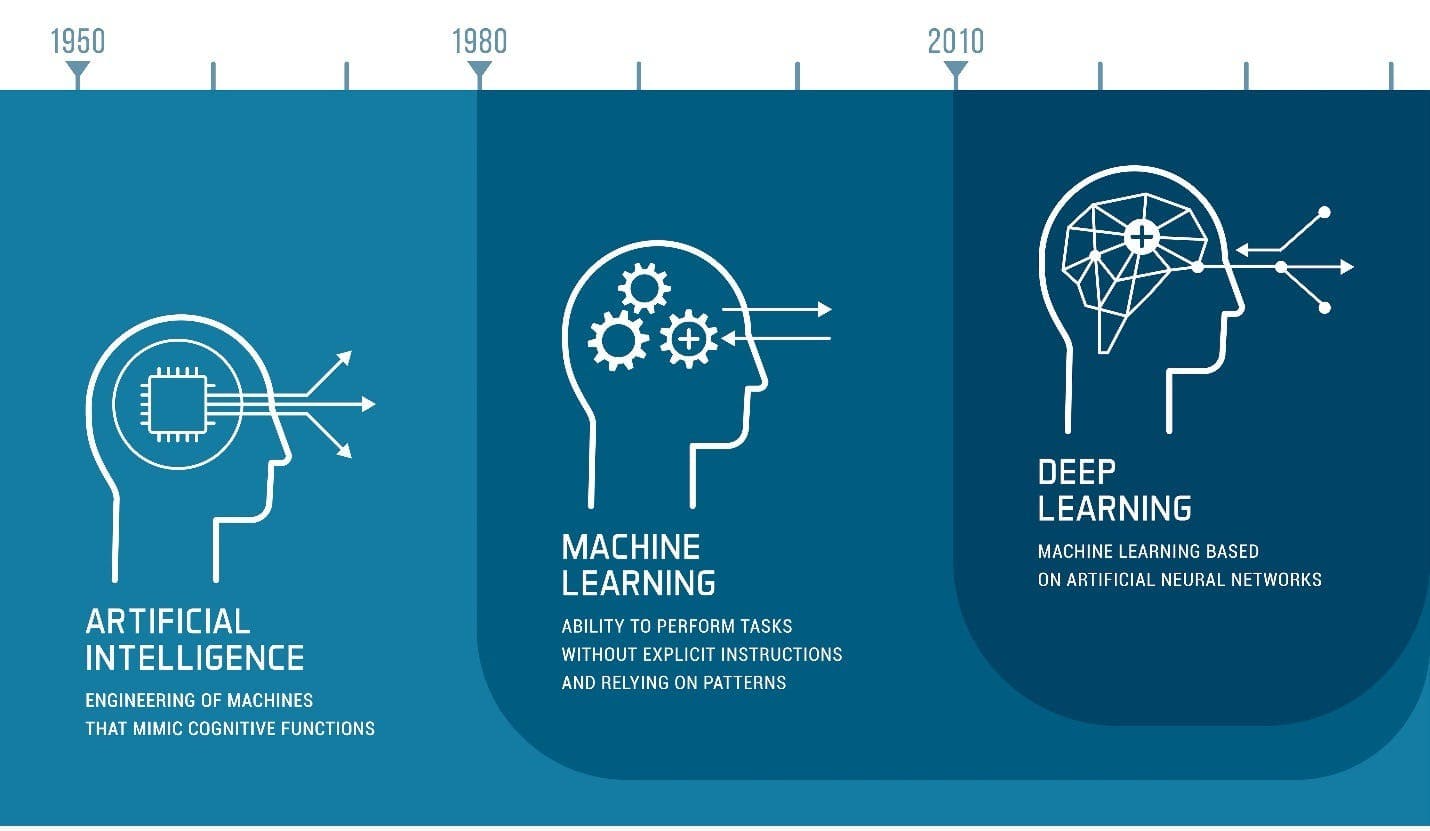
\includegraphics[scale=0.2]{history.png}
    \caption{Cronograma sobre el avance de la Inteligencia Artificial. \cite{tjk2024deep}}
\end{figure}

Mientras que los modelos de aprendizaje supervisado requieren datos de entrada estructurados y etiquetados para obtener resultados precisos, los modelos de deep learning pueden utilizar el aprendizaje no supervisado. Con el aprendizaje no supervisado, los modelos de deep learning pueden extraer las características, los rasgos y las relaciones que necesitan para obtener resultados precisos a partir de datos brutos y no estructurados. Además, estos modelos pueden incluso evaluar y refinar sus resultados para aumentar la precisión. \\

\begin{figure}[H]
    \centering
    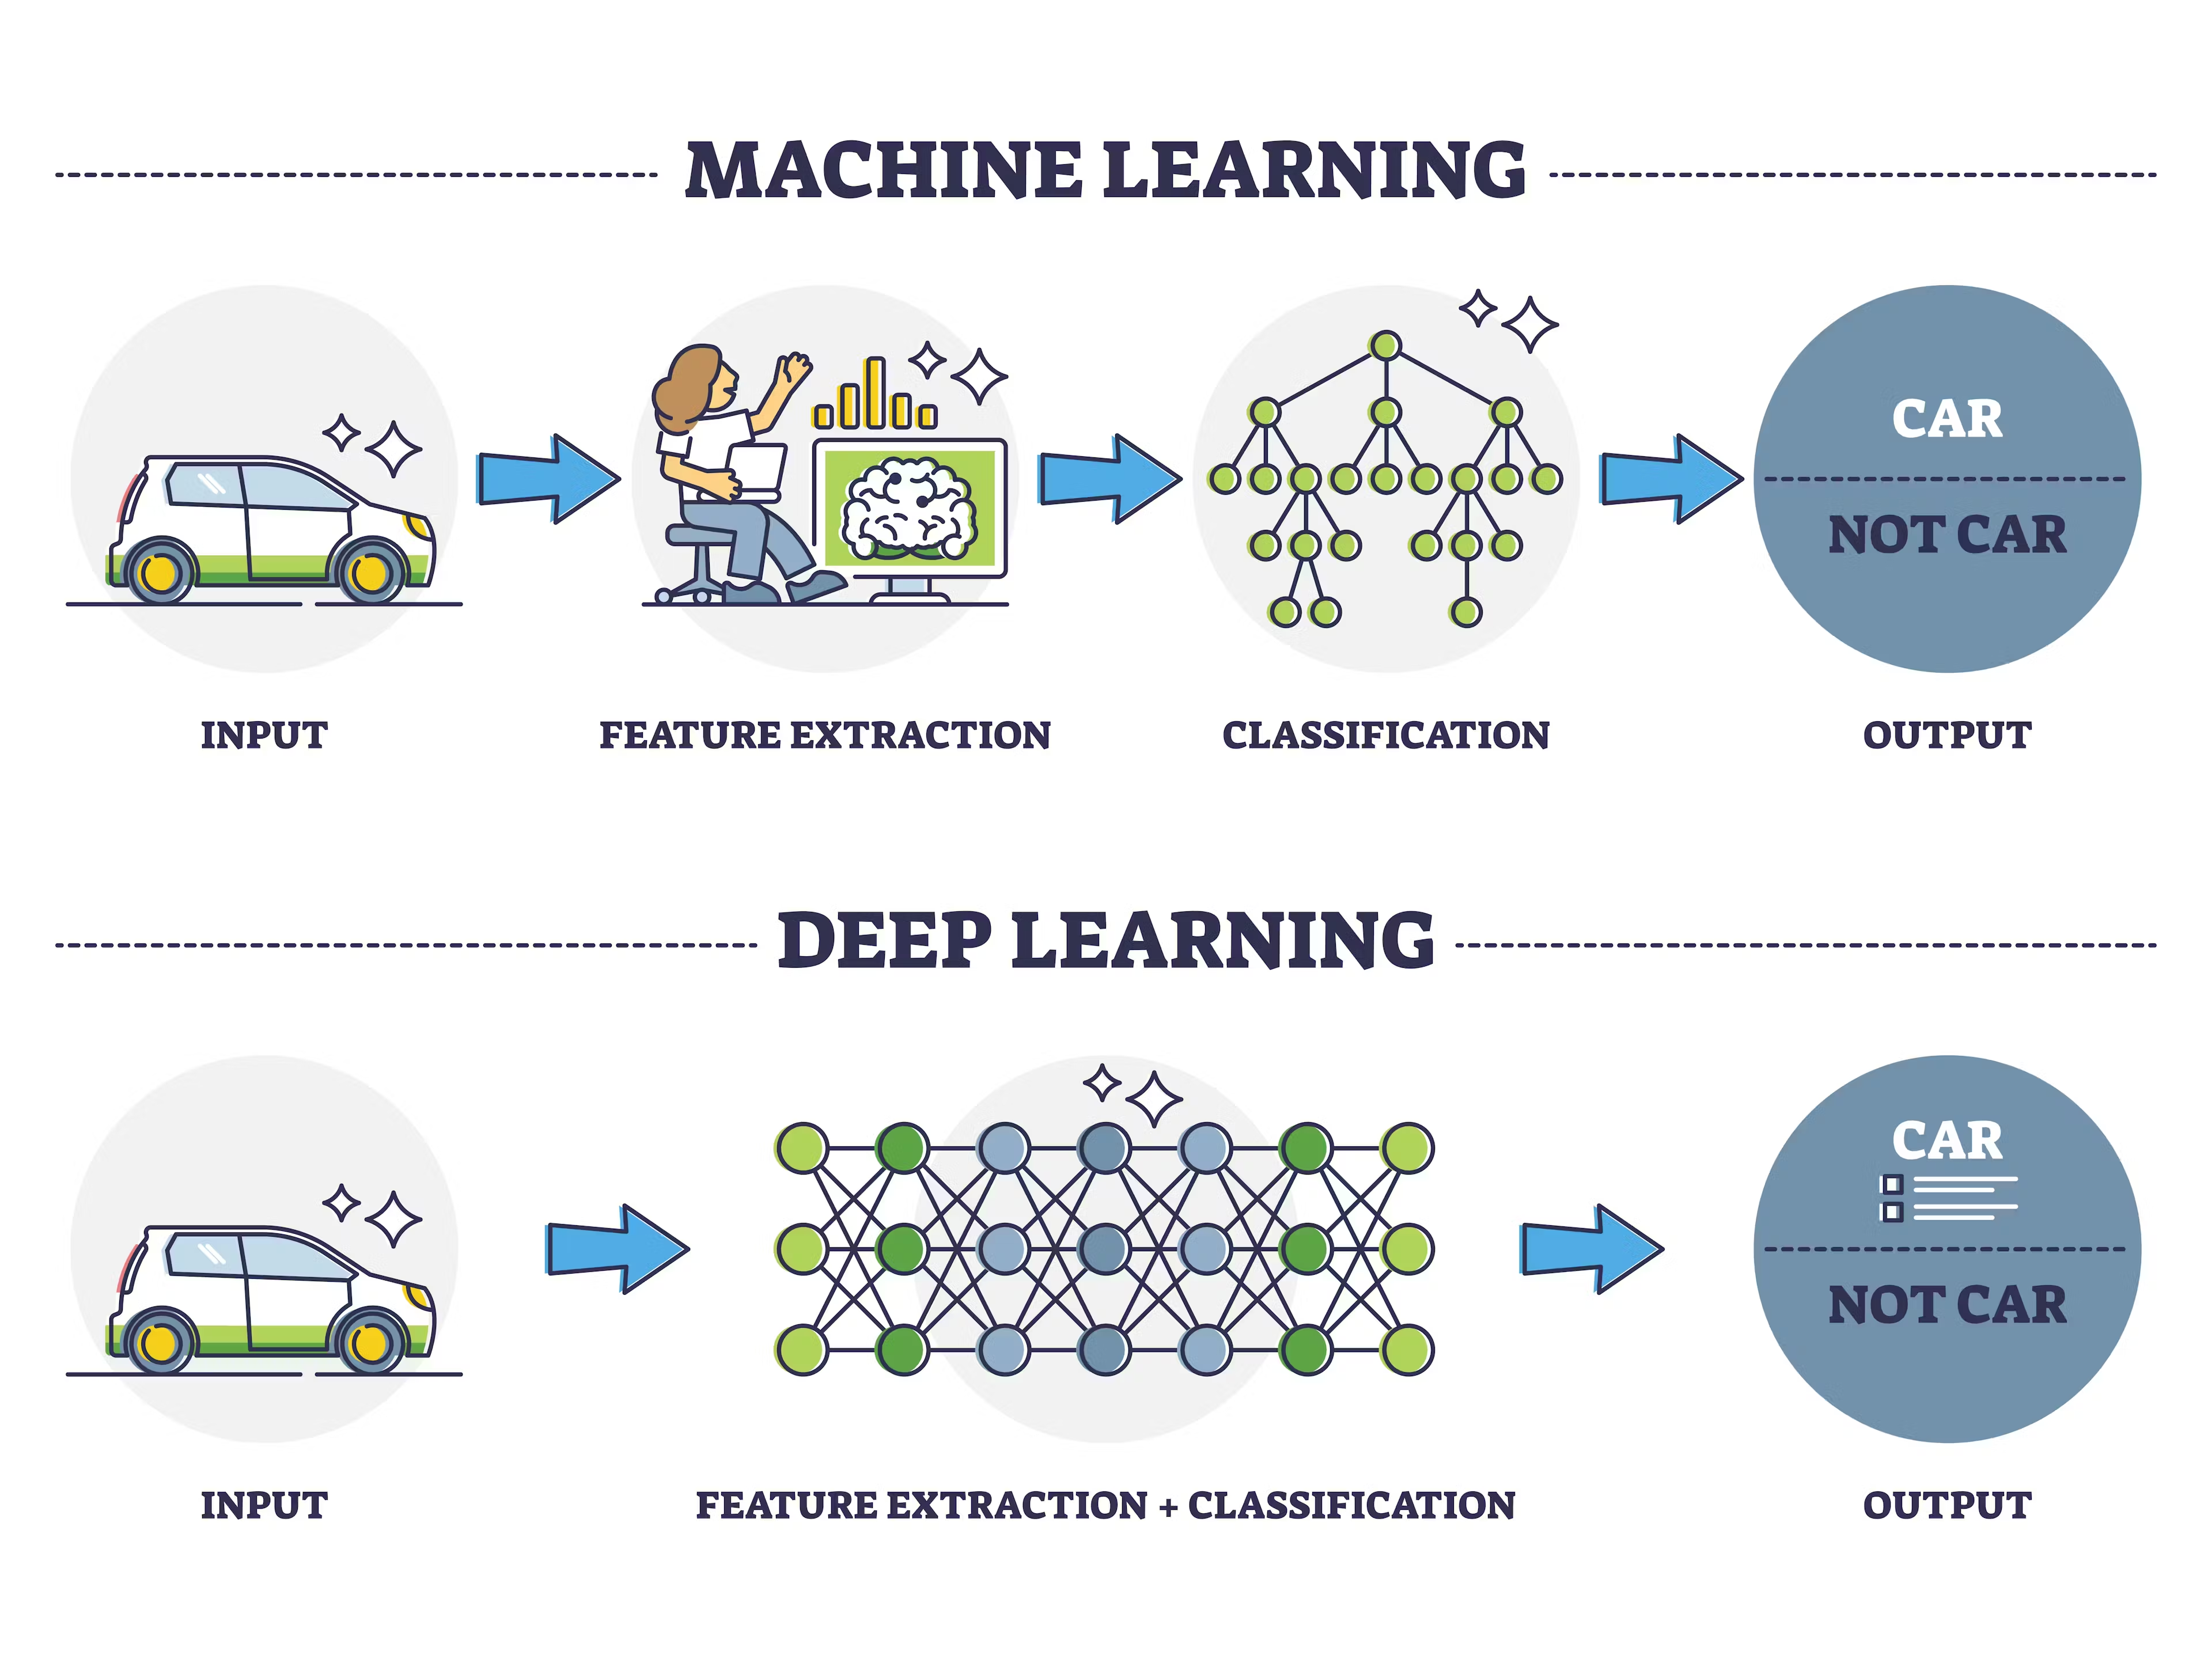
\includegraphics[scale=0.075]{mlvsdp.png}
    \caption{Machine Learning vs Deep Learning.}
\end{figure}

El deep learning es un aspecto de la ciencia de datos que impulsa muchas aplicaciones y servicios que mejoran la automatización, realizando tareas analíticas y físicas sin intervención humana. Esto permite muchos productos y servicios cotidianos, como asistentes digitales, controles remotos de TV habilitados para voz, detección de fraudes con tarjetas de crédito, automóviles autónomos e IA generativa. \\

\newpage

\subsubsection{¿Cómo funciona el Deep Learning?}
Las redes neuronales, o redes neuronales artificiales, intentan imitar el cerebro humano a través de una combinación de entradas de datos, ponderaciones y sesgos, todos actuando como neuronas de silicio. Estos elementos trabajan juntos para reconocer, clasificar y describir con precisión los objetos dentro de los datos. \\

Las redes neuronales profundas se componen de varias capas de nodos interconectados, cada una de las cuales se basa en la capa anterior para refinar y optimizar la predicción o la categorización. Esta progresión de cálculos a través de la red se denomina propagación hacia adelante. Las capas de entrada y salida de una red neuronal profunda se denominan capas visibles . La capa de entrada es donde el modelo de deep learning ingiere los datos para su procesamiento, y la capa de salida es donde se realiza la predicción o clasificación final. \\

\begin{figure}[H]
    \centering
    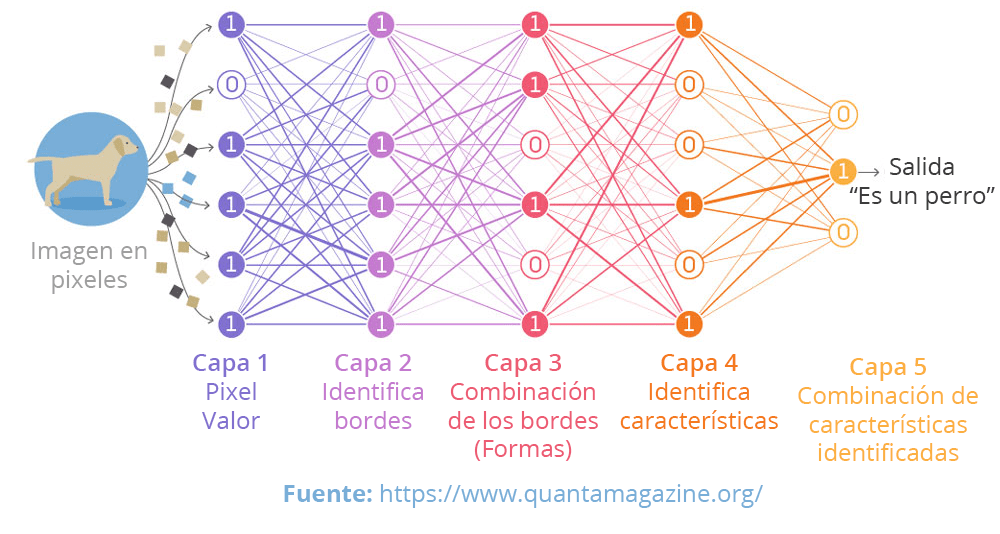
\includegraphics[scale=0.3]{layers.png}
    \caption{Red Neuronal.}
\end{figure}

El deep learning requiere una enorme cantidad de potencia informática. Las unidades de procesamiento gráfico (GPU) de alto rendimiento son ideales porque pueden manejar un gran volumen de cálculos en varios núcleos con memoria copiosa disponible. El cloud computing distribuida también podría resultar útil. Este nivel de potencia de cómputo es necesario para entrenar algoritmos profundos a través del deep learning. Sin embargo, gestionar varias GPU en las instalaciones puede generar una gran demanda de recursos internos y su escalamiento es increíblemente caro. Para los requisitos de software, la mayoría de las aplicaciones de deep learning están codificadas con uno de estos tres marcos de aprendizaje: JAX, PyTorch o TensorFlow. \\

\newpage

\subsection{Redes Neuronales Recurrentes (RNN)}
\subsubsection{¿Qué son las RNN?}
Una red neuronal recurrente, o (RNN), es una red neuronal \cite{ibm-nn} profunda entrenada con datos secuenciales o de series temporales para crear un modelo de machine learning \cite{ibm-ml} que pueda hacer predicciones secuenciales o conclusiones basadas en entradas secuenciales. \\

Una (RNN) podría utilizarse para predecir los niveles diarios de inundación basándose en los datos diarios anteriores sobre inundaciones, mareas y meteorología.
Pero las (RNN) también se pueden utilizar para resolver problemas ordinales o temporales, como la traducción de idiomas, el procesamiento del lenguaje natural (PLN) \cite{ibm-pln}, el reconocimiento de voz \cite{ibm-sr} y el subtitulado de imágenes.
Las (RNN) se incorporan a aplicaciones populares como Siri, búsqueda por voz y Google Translate.

\subsubsection{Funcionamiento de las RNN}
Al igual que [las redes neuronales convolucionales CNN \cite{ibm-cnn}, las redes neuronales recurrentes utilizan datos de entrenamiento para aprender.
Se distinguen por su ``memoria'', ya que toman la información de las entradas anteriores para influir en la entrada y la salida actuales.
Aunque las redes neuronales profundas tradicionales asumen que las entradas y las salidas son independientes entre sí, la salida de los (RNN) depende de los elementos anteriores de la secuencia.
Mientras que las redes neuronales profundas tradicionales asumen que las entradas y las salidas son independientes entre sí, la salida de las (RNN) depende de los elementos anteriores dentro de la secuencia. \\

Tomemos un modismo, como el inglés ``feeling under the weather'', que se utiliza comúnmente cuando alguien está enfermo, para ayudarnos en la explicación de las (RNN).
Para que el modismo tenga sentido, debe expresarse en ese orden específico.
En consecuencia, las redes recurrentes deben tener en cuenta la posición de cada palabra en el modismo y utilizan esa información para predecir la siguiente palabra de la secuencia.

\begin{figure}[H]
    \centering
    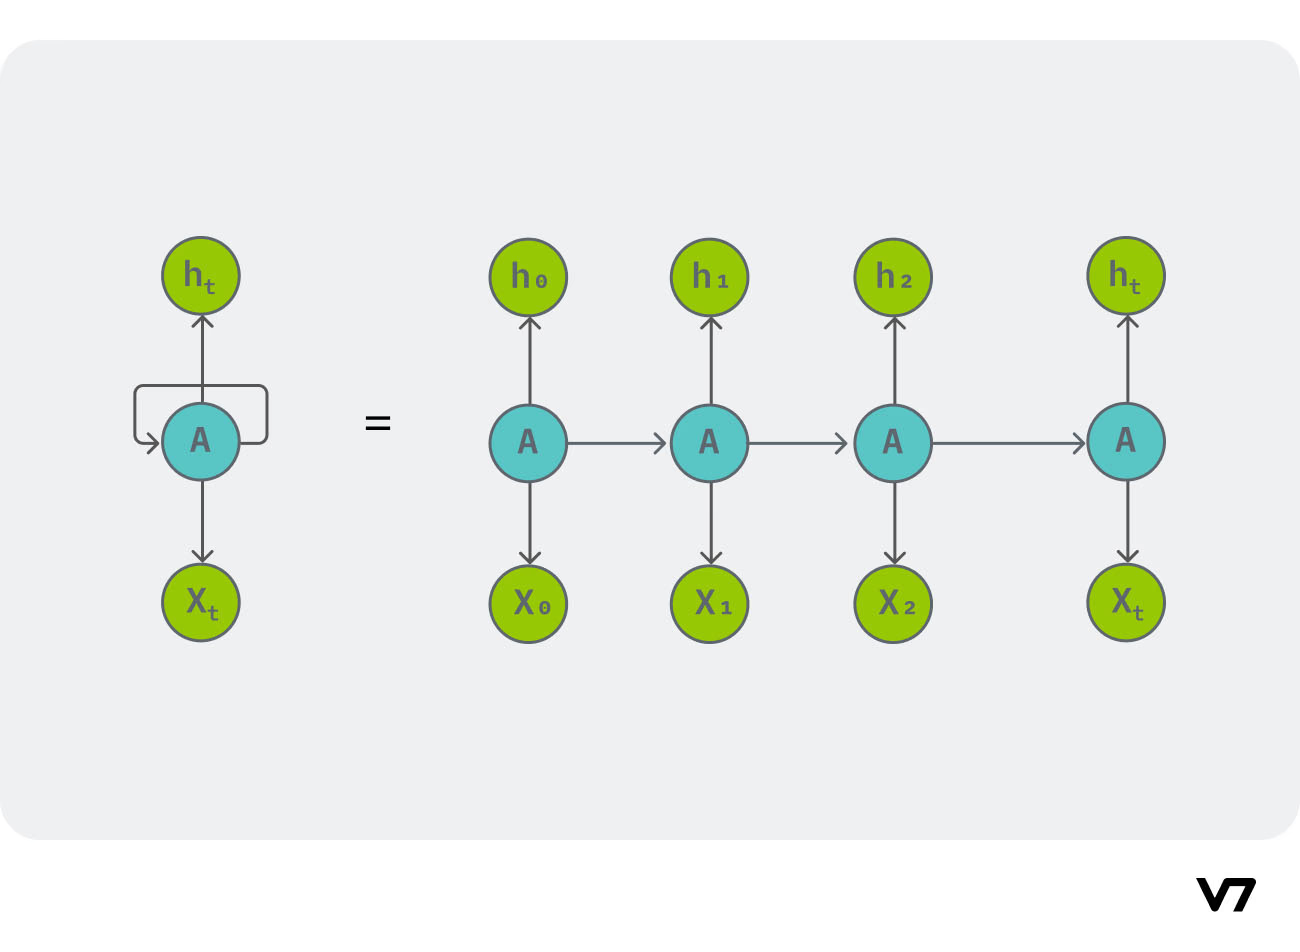
\includegraphics[scale=0.2]{secuencia.png}
    \caption{Secuencia y pesos en una RNN.}
\end{figure}

Otra característica distintiva de las redes recurrentes es que comparten parámetros en cada capa de la red.
Mientras que las redes feedforward tienen diferentes pesos en cada nodo, las redes neuronales recurrentes comparten el mismo parámetro de peso dentro de cada capa de la red.
Dicho esto, estos pesos todavía se ajustan a través de los procesos de retropropagación y descenso de gradiente para facilitar el aprendizaje por refuerzo.

\newpage

Las redes neuronales recurrentes aprovechan los algoritmos de retropropagación a través del tiempo (BPTT, por sus siglas en inglés) para determinar los gradientes, lo que difiere ligeramente de la retropropagación tradicional, ya que es específica de los datos secuenciales.
Los principios de la (BPTT) son los mismos que los de la retropropagación tradicional, en la que el modelo se entrena a sí mismo calculando los errores de su capa de salida a su capa de entrada.
Estos cálculos nos permiten ajustar y ajustar los parámetros del modelo adecuadamente.
(BPTT) difieren del enfoque tradicional en que estas suman errores en cada paso de tiempo mientras que las redes feedforward no necesitan sumar errores ya que no comparten parámetros a través de cada capa.

\begin{figure}[H]
    \centering
    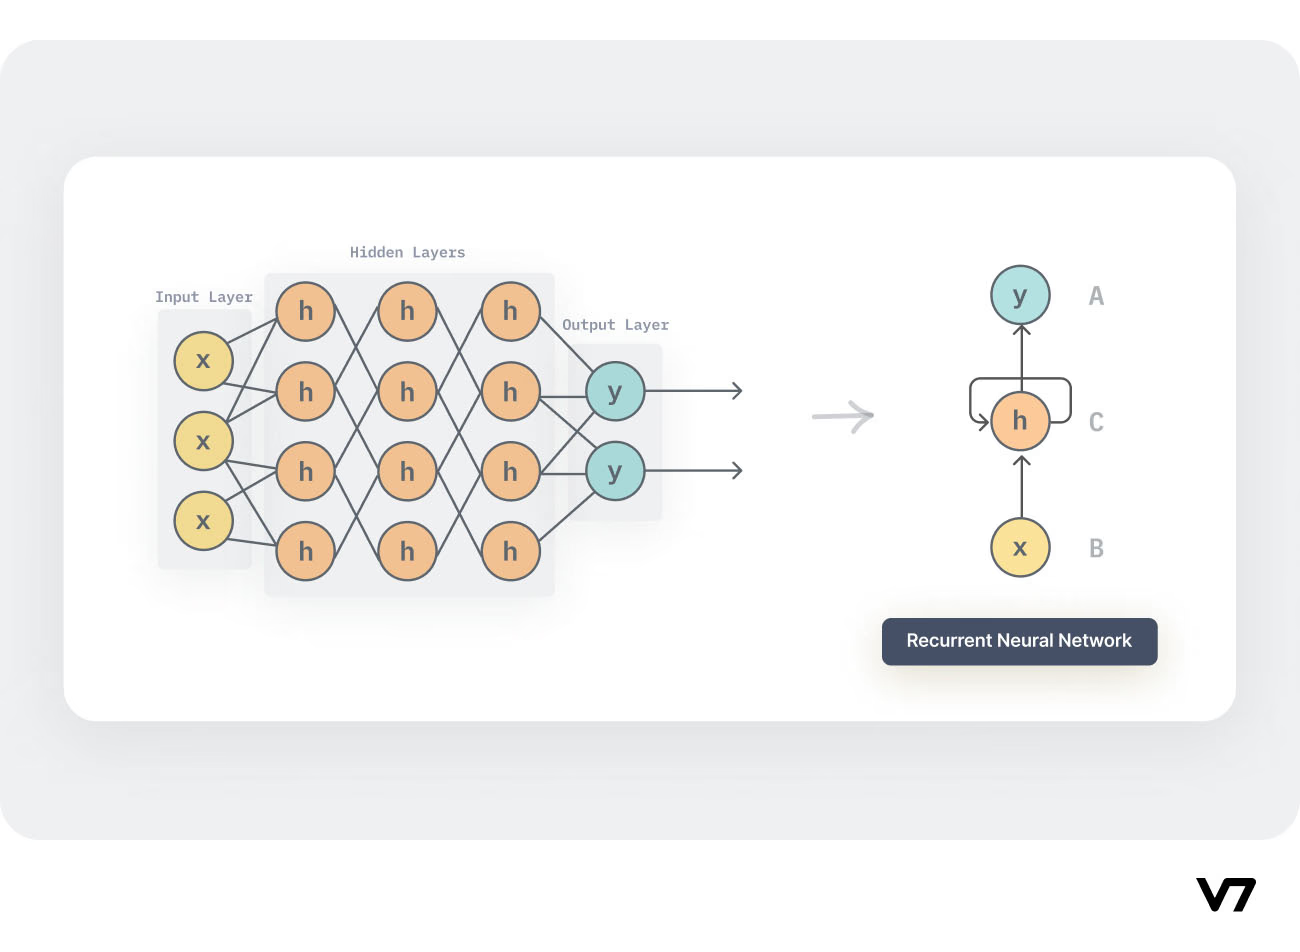
\includegraphics[scale=0.25]{capas.png}
    \caption{Capas en una red neuronal.}
\end{figure}

Durante este proceso, las (RNN) tienden a enfrentarse a dos problemas, conocidos como gradientes de explosión y gradientes de desaparición.
Estos problemas se definen por el tamaño del gradiente, que es la pendiente de la función de pérdida a lo largo de la curva de error.
Cuando el gradiente es demasiado pequeño, sigue haciéndose más pequeño, actualizando los parámetros de peso hasta que se vuelven insignificantes, es decir, cuando eso ocurre, el algoritmo ya no está aprendiendo.
La explosión de gradientes sucede cuando el gradiente es demasiado grande, lo que crea un modelo inestable.
En este caso, los pesos del modelo crecerán demasiado y, finalmente, se representarán como \textit{NaN}.
Una solución a estos problemas es reducir el número de capas ocultas de la red neuronal, lo que elimina parte de la complejidad de los modelos (RNN).

\begin{figure}[H]
    \centering
    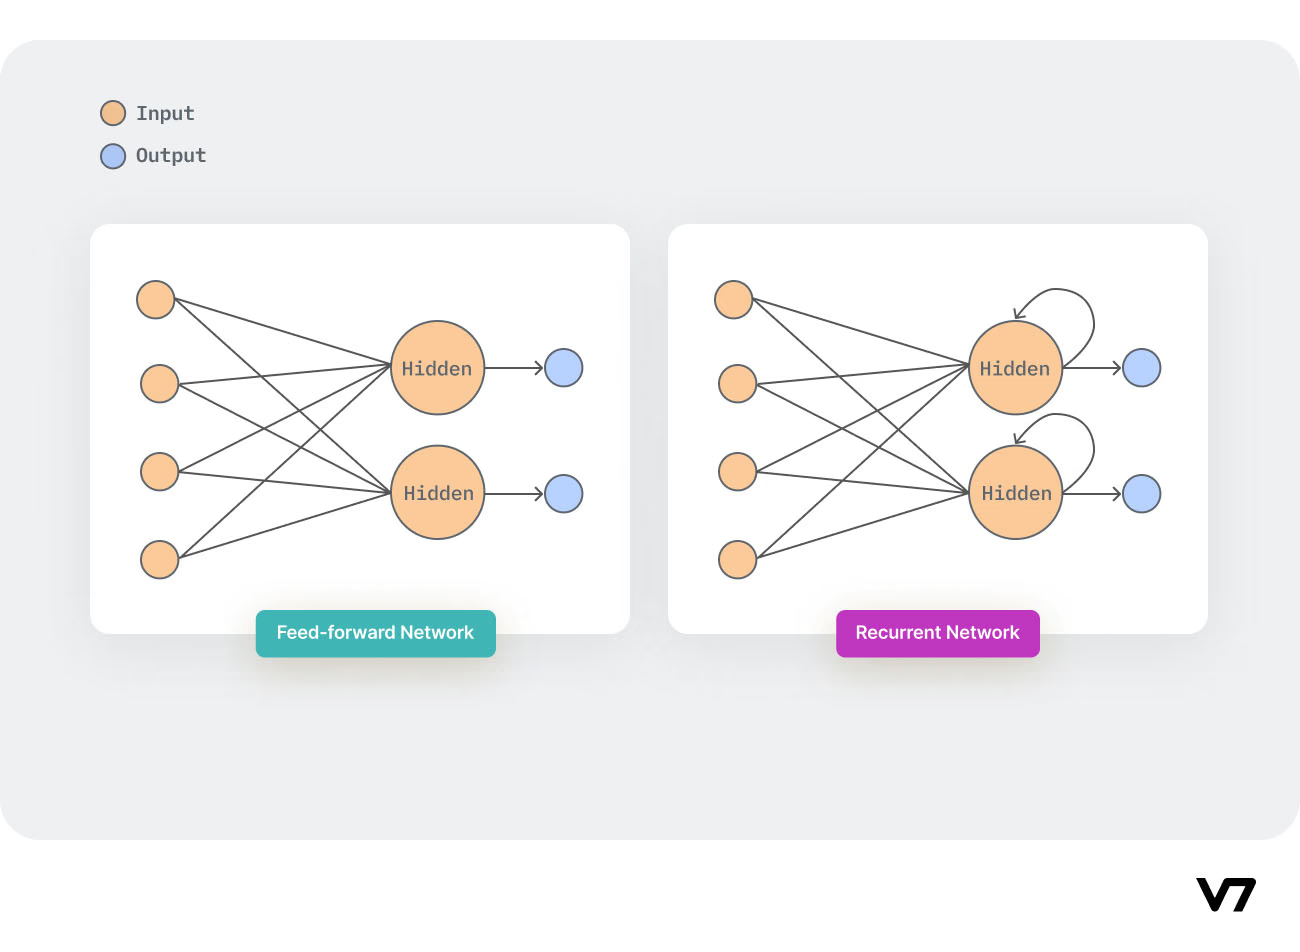
\includegraphics[scale=0.25]{ffrn.png}
    \caption{Feed-Forward Network vs Recurrent Network.}
\end{figure}

\newpage

\subsubsection{Tipos de RNN}
Las redes neuronales tradicionales tienen capas de entrada y salida independientes, lo que las hace inadecuadas para manejar datos secuenciales.
Las Redes Neuronales Recurrentes (RNN) se introdujeron para almacenar los resultados de salidas previas en una memoria interna.
Los cuatro tipos más comúnmente utilizados de Redes Neuronales Recurrentes son:

\begin{itemize}
    \item \textbf{One-To-One}: El tipo más simple de (RNN) es el One-to-One, que permite una sola entrada y una sola salida. Tiene tamaños de entrada y salida fijos, y actúa como una red neuronal estándar. Una de las aplicaciones del modelo One-to-One se encuentra en la clasificación de imágenes.
\end{itemize}

\begin{figure}[H]
    \centering
    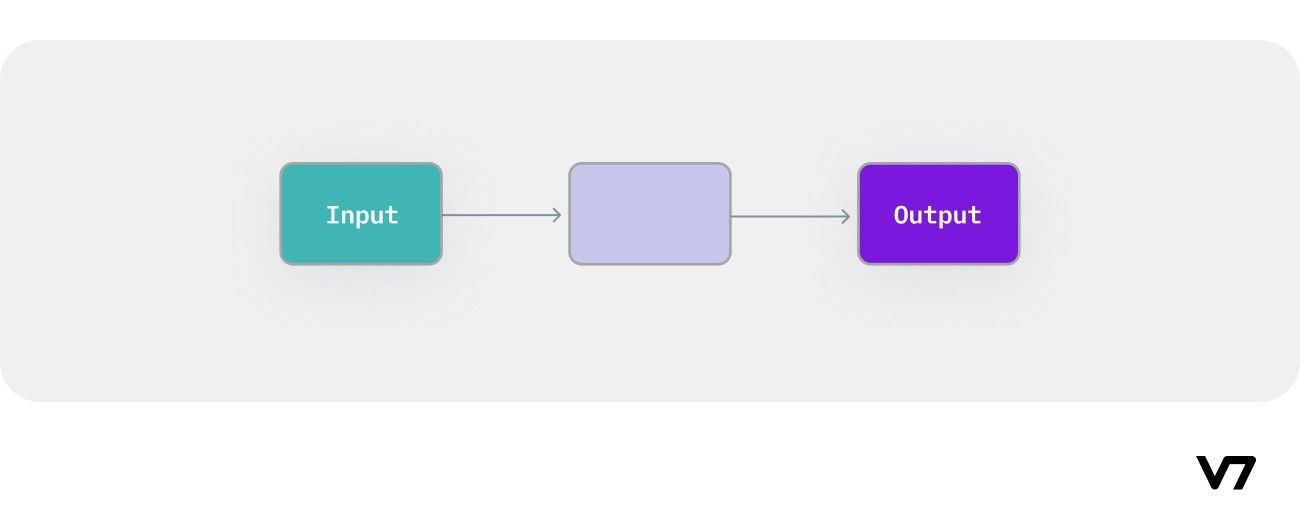
\includegraphics[scale=0.25]{oto.jpeg}
    \caption{One-To-One.}
\end{figure}

\begin{itemize}
    \item \textbf{One-To-Many}: El One-to-Many es un tipo de (RNN) que genera múltiples salidas a partir de una única entrada proporcionada al modelo. El tamaño de la entrada es fijo y produce una serie de datos como salida. Sus aplicaciones se encuentran en áreas como la generación de música y la generación de descripciones para imágenes (Image Captioning).
\end{itemize}

\begin{figure}[H]
    \centering
    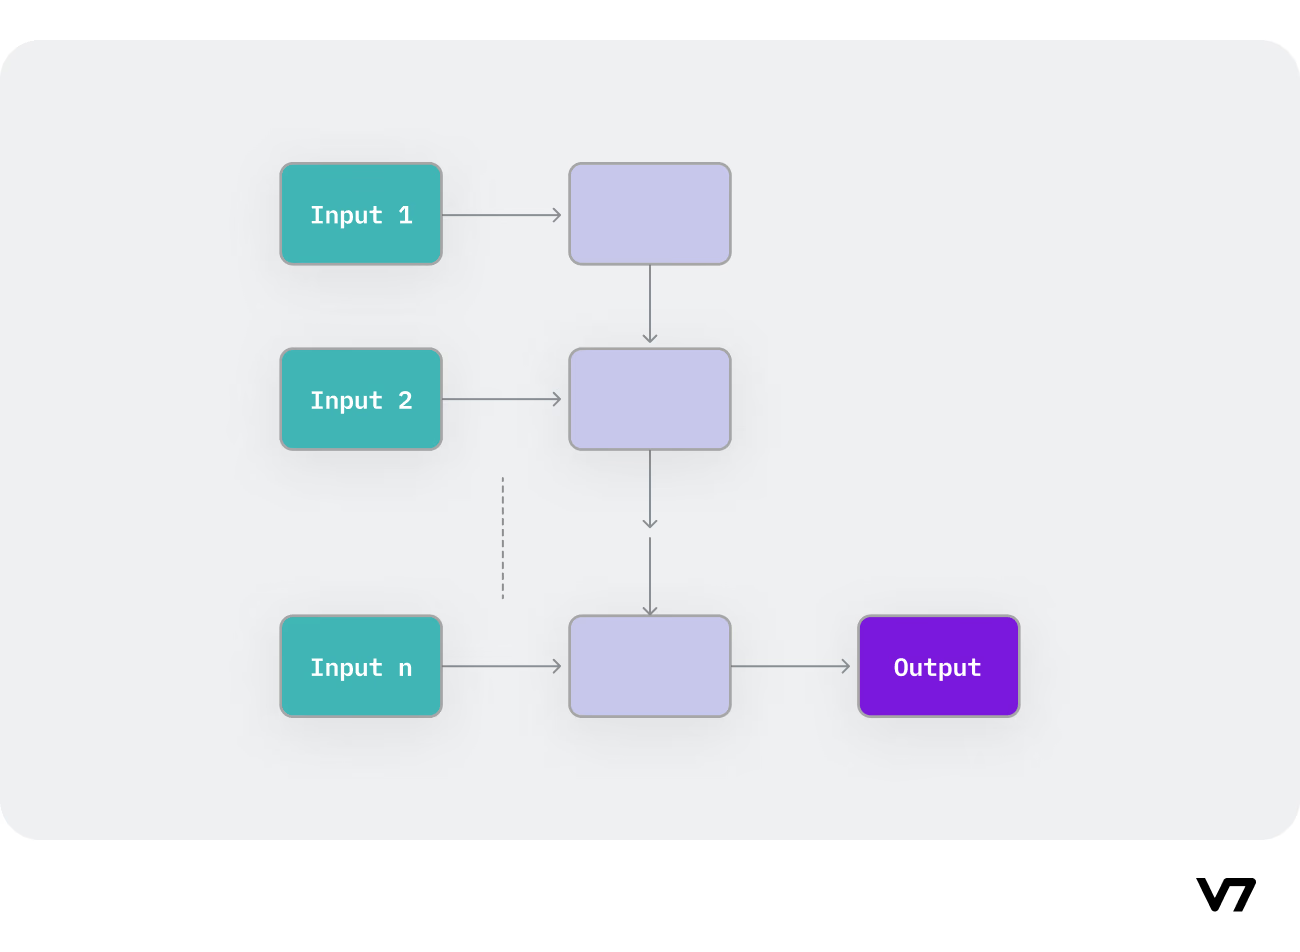
\includegraphics[scale=0.25]{mto.png}
    \caption{One-To-Many.}
\end{figure}

\newpage

\begin{itemize}
    \item \textbf{Many-To-Many}: es un tipo de RNN que se utiliza para generar una secuencia de datos de salida a partir de una secuencia de unidades de entrada. Este tipo se divide en las siguientes dos subcategorías:
    \begin{itemize}
        \item \textbf{Equal-Size}: En este caso, el tamaño de las capas de entrada y salida es exactamente el mismo.
    \end{itemize}
    \begin{figure}[H]
        \centering
        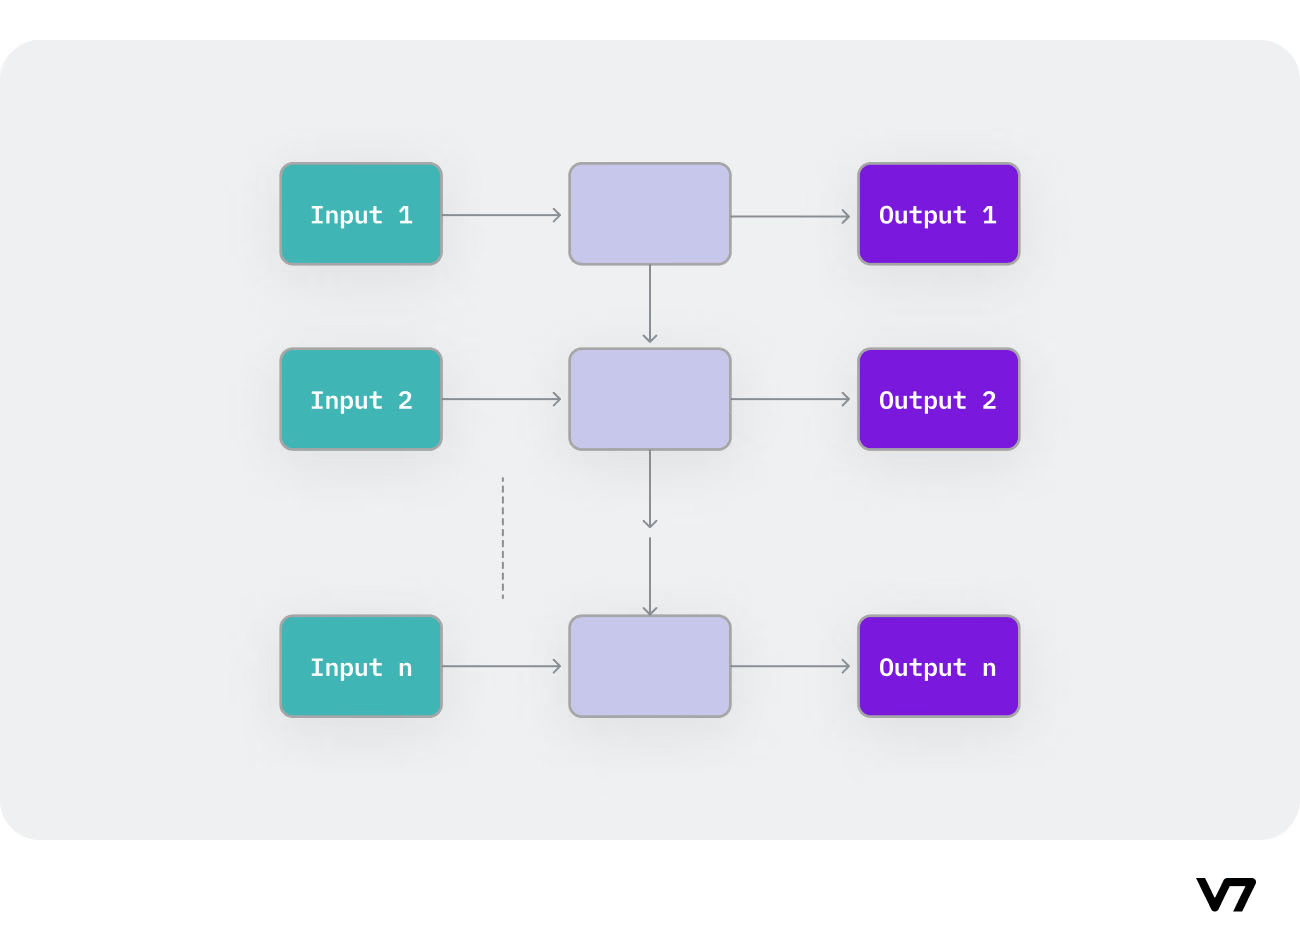
\includegraphics[scale=0.25]{mteq.png}
        \caption{Many-To-Many (Equal-Size).}
    \end{figure}
    \begin{itemize}
        \item \textbf{Unequal-Size}: En este caso, las entradas y salidas tienen un número diferente de unidades. Su aplicación se encuentra en la \textit{traducción automática} (Machine Translation).
    \end{itemize}
    \begin{figure}[H]
        \centering
        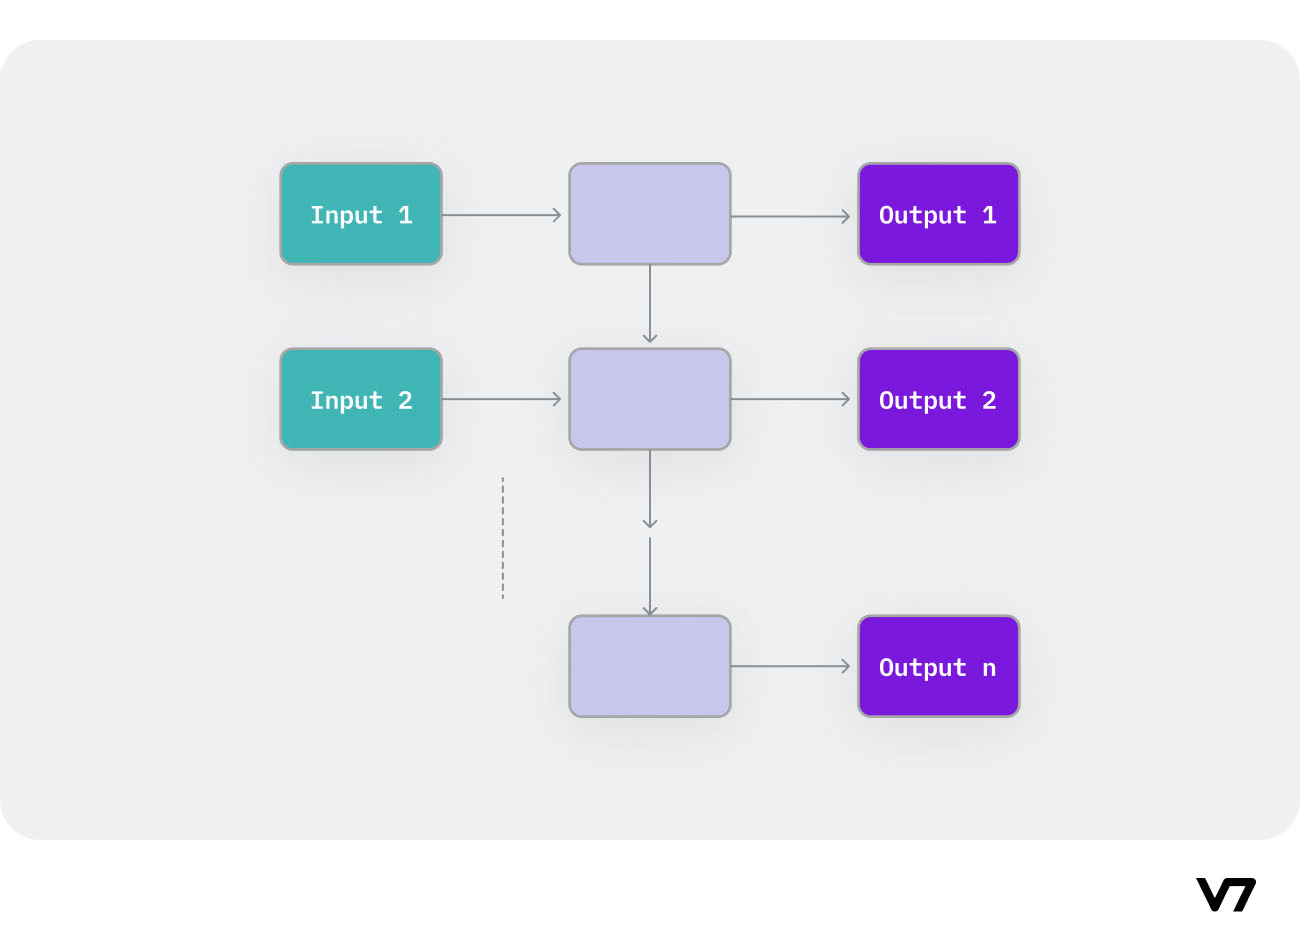
\includegraphics[scale=0.25]{mtun.png}
        \caption{Many-To-Many (Unequal-Size).}
    \end{figure}
\end{itemize}

\subsection{Arquitecturas RNN variantes}
\subsubsection{Redes neuronales recurrentes bidireccionales (BRNN)}
Mientras que en las RNN unidireccionales sólo se pueden extraer de entradas anteriores para hacer predicciones sobre el estado actual, las RNN bidireccionales, o BRNN, extraen datos futuros para mejorar la precisión de los mismos. Volviendo al ejemplo de ``feeling under the weather'', un modelo basado en una BRNN puede predecir mejor que la segunda palabra de esa frase es ``under'' si sabe que la última palabra de la secuencia es ``weather''.

\begin{figure}[H]
    \centering
    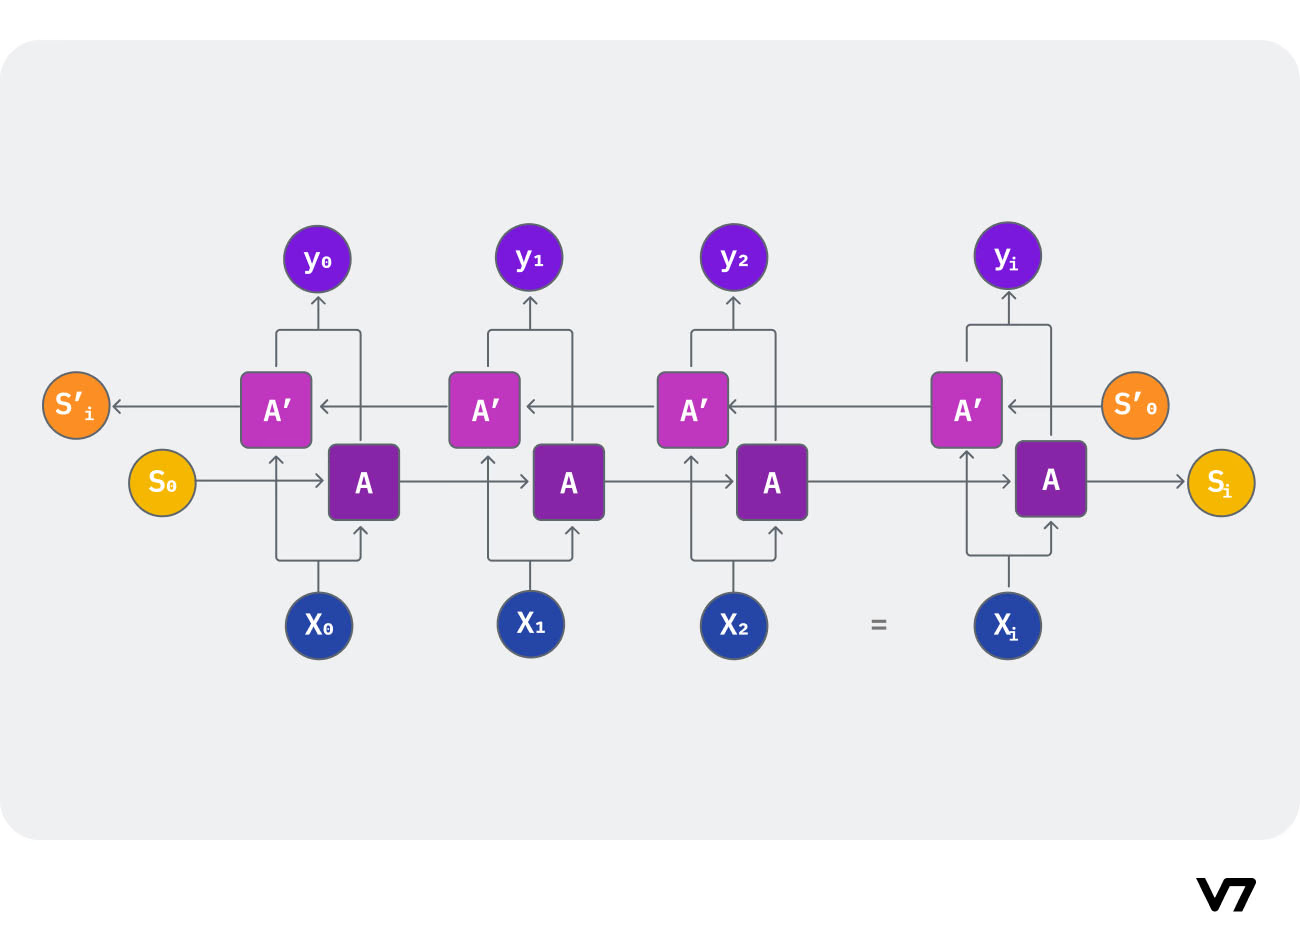
\includegraphics[scale=0.25]{brnn.png}
    \caption{Red Neuronal Recurrente Bidireccional.}
\end{figure}

\newpage

\subsubsection{Memoria a corto y largo plazo (LSTM)}
LSTM es una arquitectura RNN popular, que fue introducida por Sepp Hochreiter y Juergen Schmidhuber como una solución al problema del gradiente evanescente. En su artículo \cite{lstmpaper} trabajan para abordar el problema de las dependencias a largo plazo. Es decir, si el estado anterior que influye en la predicción actual no se encuentra en el pasado reciente, es posible que el modelo RNN no pueda predecir con exactitud el estado actual. \\

Por ejemplo, supongamos que queremos predecir las palabras en cursiva que siguen: ``Alicia es alérgica a los frutos secos. No puede comer mantequilla de cacahuete''. El contexto de una alergia a los frutos secos puede ayudarnos a anticipar que los alimentos que no se pueden comer contienen frutos secos. Sin embargo, si ese contexto estuviera unas frases antes, dificultaría, o incluso imposibilitaría, que la RNN conectara la información. \\

Para solucionarlo, las LSTM tienen ``celdas'' en las capas ocultas de la red neuronal, que tienen tres puertas: una puerta de entrada, una puerta de salida y una puerta de olvido. Estas puertas controlan el flujo de información que se necesita para predecir la salida en la red. Por ejemplo, si los pronombres de género, como ``ella'', se repitieron varias veces en oraciones anteriores, puede excluirlos del estado de la celda. \\

\begin{figure}[H]
    \centering
    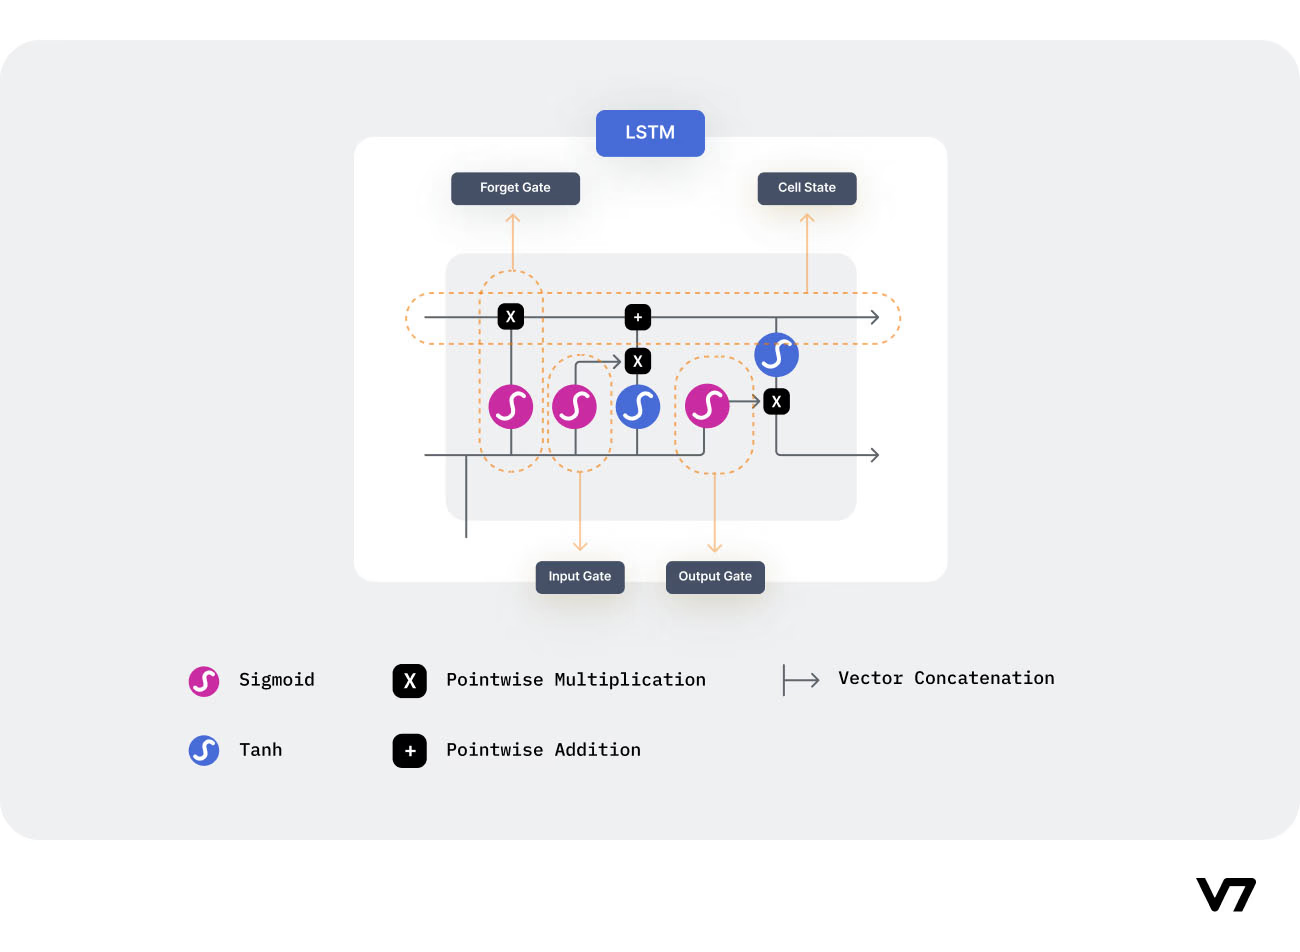
\includegraphics[scale=0.3]{lstm.png}
    \caption{Memoria a Corto y Largo Plazo.}
\end{figure}

\newpage

\subsubsection{Unidades recurrentes bloqueadas (GRU)}
Pueden darse escenarios en los que aprender únicamente de los datos inmediatamente anteriores en una secuencia sea insuficiente. Consideremos el caso de intentar predecir una frase basada en otra frase introducida mucho antes en un libro o artículo. En este caso, recordar tanto los datos inmediatamente precedentes como los anteriores resulta crucial. Una RNN, debido a su mecanismo de compartición de parámetros, utiliza los mismos pesos en cada paso de tiempo. Como resultado, la retropropagación puede hacer que el gradiente explote o se desvanezca, y la red neuronal no aprende mucho de los datos que están alejados de la posición actual. \\

Las GRU utilizan dos puertas: la puerta de actualización (update gate) y la puerta de reinicio (reset gate). Básicamente, estas son dos vectores que deciden qué información debe pasarse a la salida. Lo especial de estas puertas es que pueden entrenarse para conservar información a largo plazo sin degradarla con el tiempo o para eliminar información irrelevante para la predicción.

\begin{itemize}
    \item \textbf{Puerta de actualización}: es responsable de determinar la cantidad de información previa que debe pasar al siguiente estado.
    \item \textbf{Puerta de reinicio}: se usa para decir cuánta información del pasado debe ser ignorada por el modelo.
\end{itemize}

\begin{figure}[H]
    \centering
    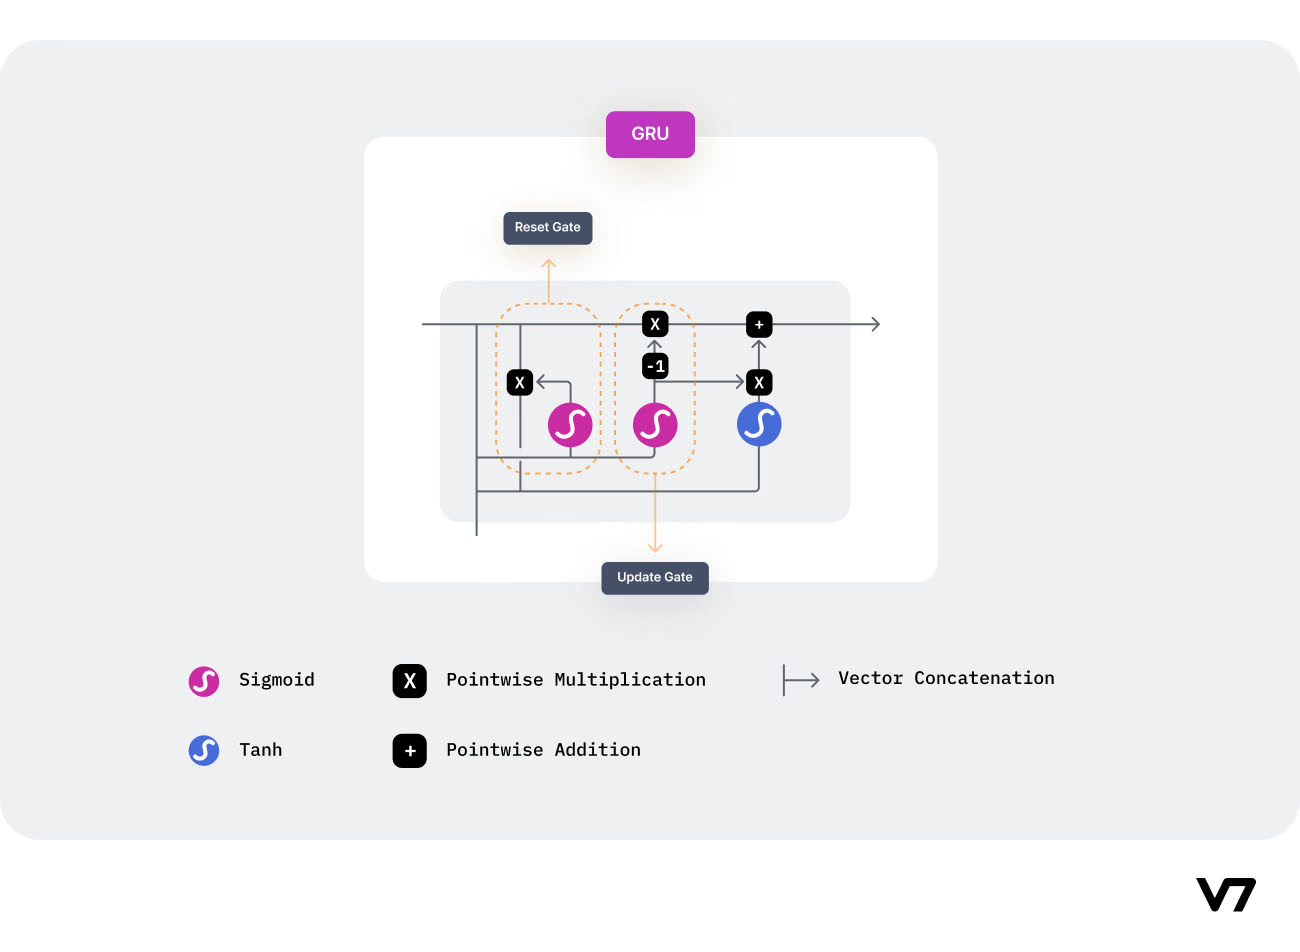
\includegraphics[scale=0.3]{gru.png}
    \caption{Unidades Recurrentes Bloqueadas.}
\end{figure}

\newpage

\subsection{Desafíos de las RNN estándar}
Entrenar una RNN, o cualquier red neuronal, se realiza definiendo una función de pérdida que mide el error o la desviación entre el valor predicho y la verdad fundamental (\textbf{ground truth}). Las características de entrada se procesan a través de múltiples capas ocultas que utilizan diferentes o las mismas funciones de activación, y se predice el resultado. La función de pérdida total se calcula, marcando así el final de la \textit{pasada hacia adelante} (\textbf{forward pass}). \\

La segunda parte del entrenamiento es la \textit{pasada hacia} atrás (\textbf{backward pass}), donde se calculan las diversas derivadas. Este proceso se vuelve aún más complejo en las Redes Neuronales Recurrentes (RNN), ya que estas procesan datos secuenciales o dependientes del tiempo. El modelo debe retropropagar los gradientes no solo a través de todas las capas ocultas, sino también a través del tiempo. Por lo tanto, en cada paso de tiempo, tiene que sumar todas las contribuciones anteriores hasta el instante de tiempo actual. \\

\begin{itemize}
    \item \textbf{Gradientes Explosivos}: En algunos casos, los valores de los gradientes continúan aumentando hasta alcanzar el infinito de forma exponencialmente rápida. Esto provoca actualizaciones de pesos muy grandes y hace que el descenso de gradiente diverja, volviendo el proceso de entrenamiento extremadamente inestable. Este problema se conoce como el gradiente explosivo (exploding gradient).
    \item \textbf{Gradientes desvanecidos}: En otros casos, a medida que la retropropagación avanza desde la capa de salida hacia la capa de entrada, el término del gradiente tiende a cero de forma exponencialmente rápida. Como resultado, los pesos de las capas iniciales o más profundas apenas cambian, lo que dificulta que el modelo aprenda dependencias de largo plazo. Esto provoca que el descenso de gradiente nunca converja al óptimo. Este problema se conoce como el gradiente desvanecido (vanishing gradient).
\end{itemize}

\newpage

\section{Preparación del Entorno}
Para la programación en Python, utilizaremos el entorno de desarrollo de JetBrains PyCharm \footnote{\url{https://www.jetbrains.com/pycharm/download/?section=windows}}.

\subsection{Pasos para la instalación}
\begin{figure}[H]
    \centering
    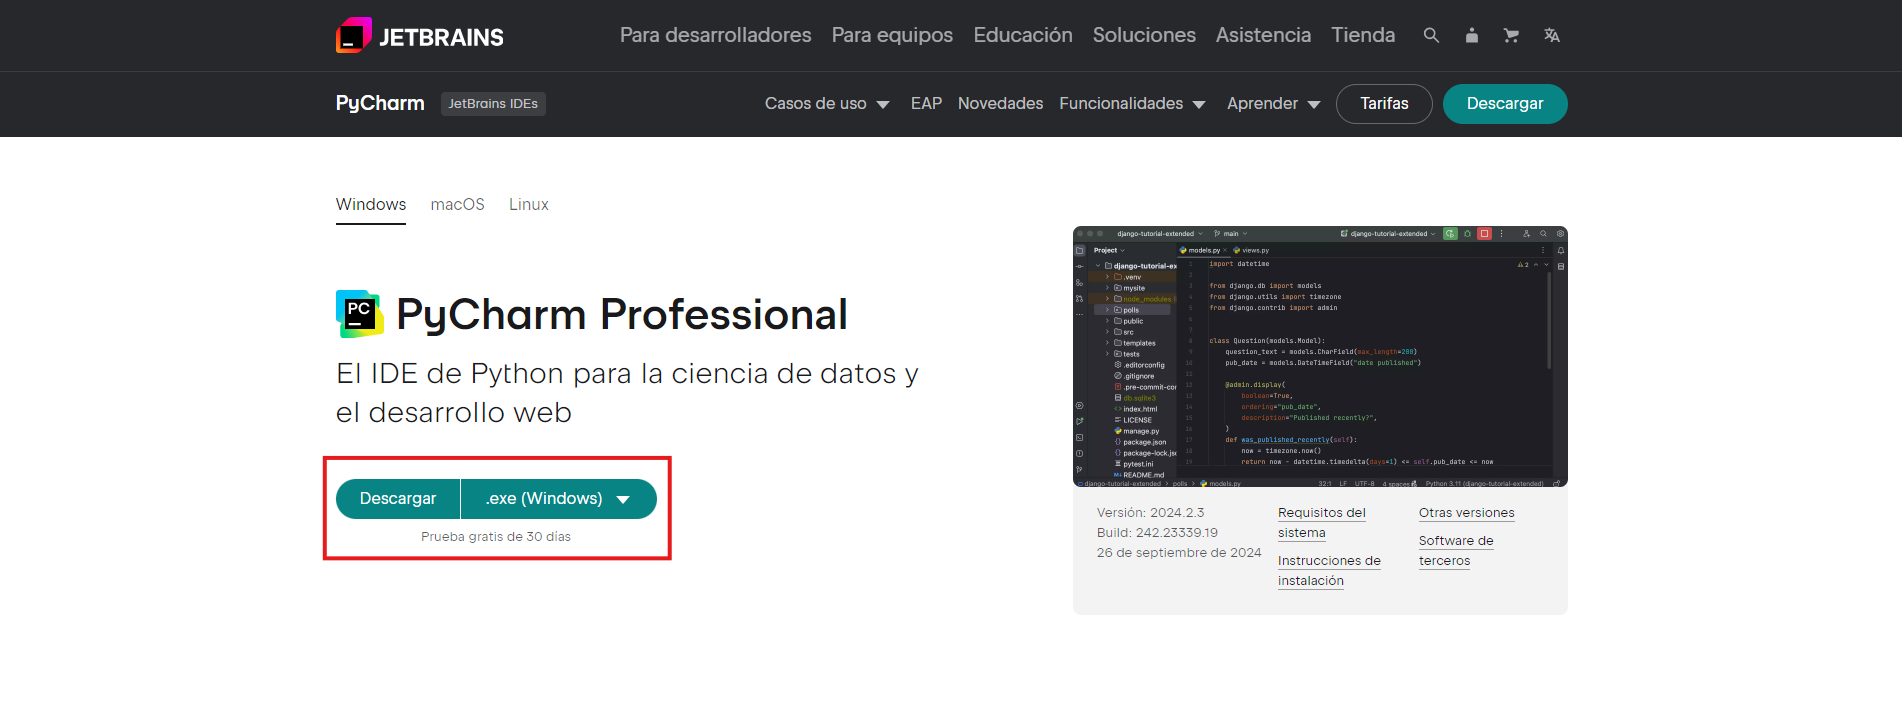
\includegraphics[scale=0.3]{py1.png}
    \caption{Descarga del archivo de instalación.}
\end{figure}

\begin{figure}[H]
    \centering
    
\includegraphics[scale=0.8]{py2.png}
    \caption{Inicio del asistente de instalación.}
\end{figure}

\begin{figure}[H]
    \centering
    
\includegraphics[scale=0.8]{py3.png}
    \caption{Seleccionar la ruta de instalación.}
\end{figure}

\begin{figure}[H]
    \centering
    
\includegraphics[scale=0.8]{py4.png}
    \caption{Seleccionar asociaciones para los ficheros.}
\end{figure}

\begin{figure}[H]
    \centering
    
\includegraphics[scale=0.8]{py5.png}
    \caption{Inicio del proceso de instalación.}
\end{figure}

\begin{figure}[H]
    \centering
    
\includegraphics[scale=0.8]{py6.png}
    \caption{Reiniciar para completar la instalación.}
\end{figure}

\begin{figure}[H]
    \centering
    
\includegraphics[scale=0.65]{py7.png}
    \caption{Página inicial de PyCharm.}
\end{figure}

\newpage

Para obtener el proyecto donde se ubica el programa, hay que ir al enlace del repositorio de GitHub \footnote{\url{https://github.com/d2nt4/deep-learning.git}} y descargarlo en formato ZIP o bien clonarlo con Git.

\begin{figure}[H]
    \centering
    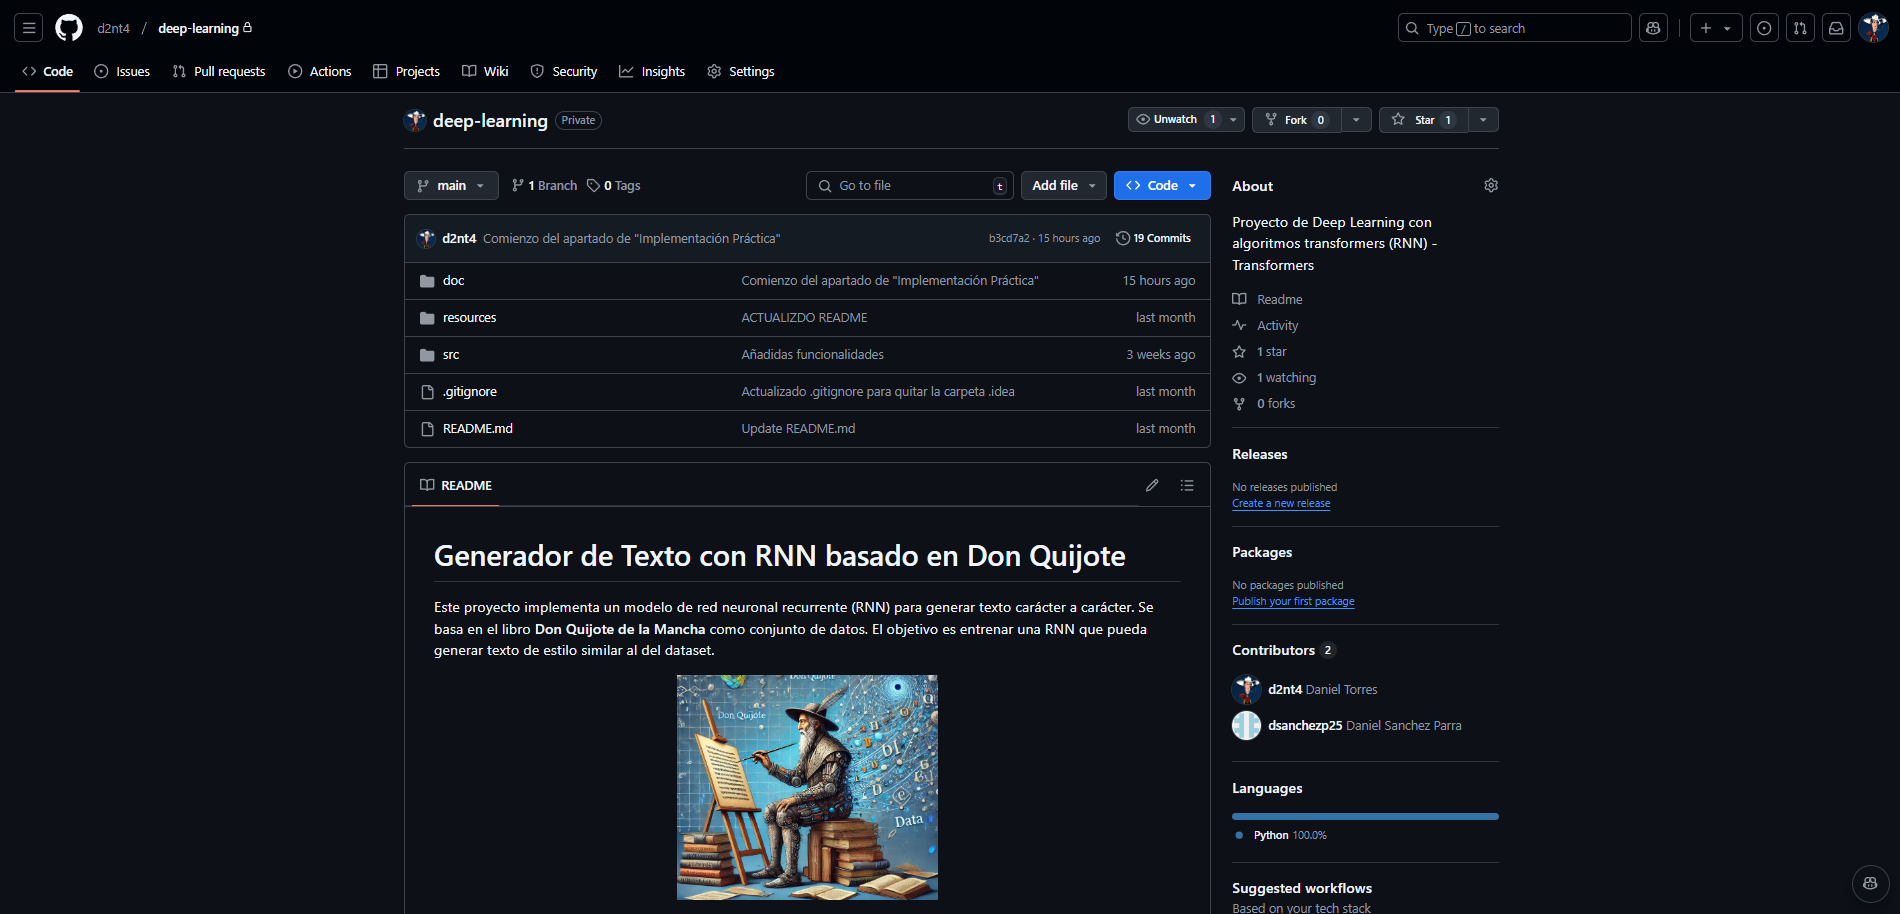
\includegraphics[scale=0.3]{github-repo.png}
    \caption{Repositorio de GitHub.}
\end{figure}

Ahora, se abre PyCharm y se procede a Abrir el proyecto ubicado en el directorio:

\begin{figure}[H]
    \centering
    
\includegraphics[scale=0.6]{py8.png}
    \caption{Abrir proyecto en PyCharm.}
\end{figure}

\begin{figure}[H]
    \centering
    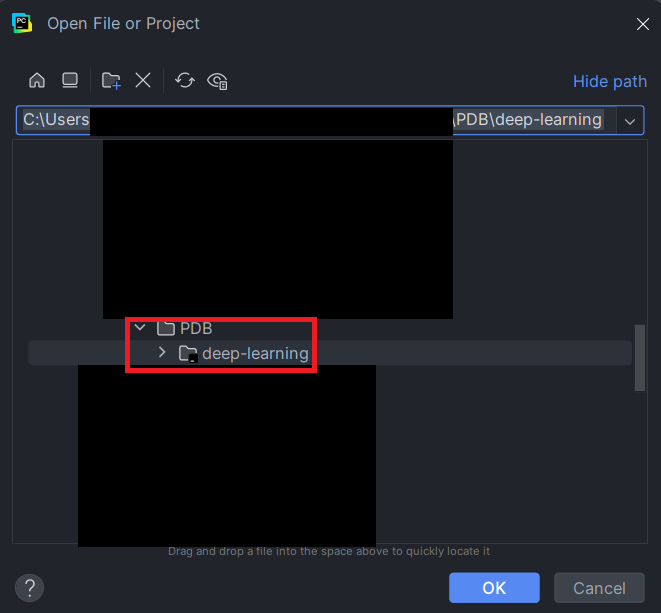
\includegraphics[scale=0.5]{py9.png}
    \caption{Seleccionar el directorio del proyecto.}
\end{figure}

Una vez abierto el proyecto, si es la primera vez, saldrá error en las librerías, pues se deben instalar. \\

Haciendo click, aparece una bombilla roja, se hace click, y aparece la opción de instalar paquete.

\begin{figure}[H]
    \centering
    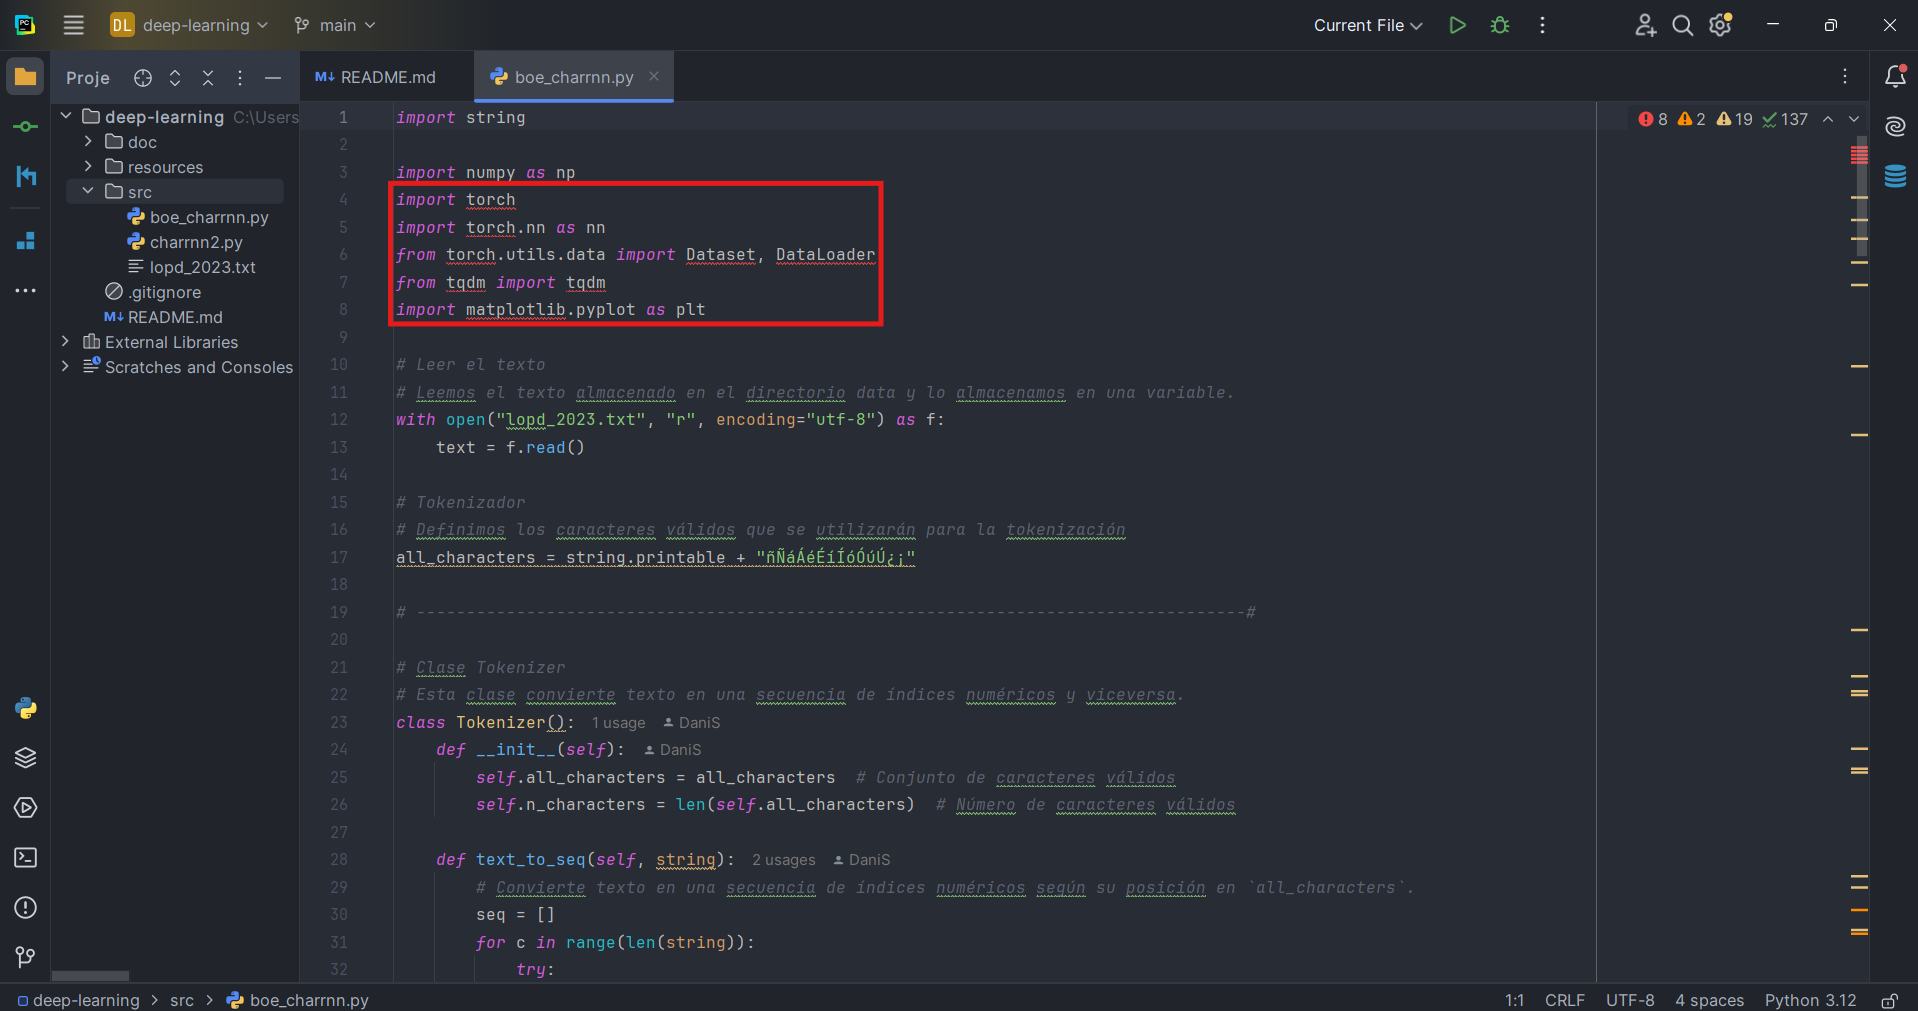
\includegraphics[scale=0.4]{py10.png}
    \caption{Instalar paquete.}
\end{figure}

\begin{figure}[H]
    \centering
    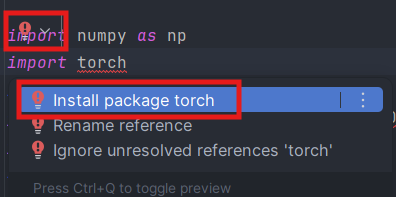
\includegraphics[scale=0.95]{py11.png}
    \caption{Seleccionar paquete a instalar.}
\end{figure}

\begin{figure}[H]
    \centering
    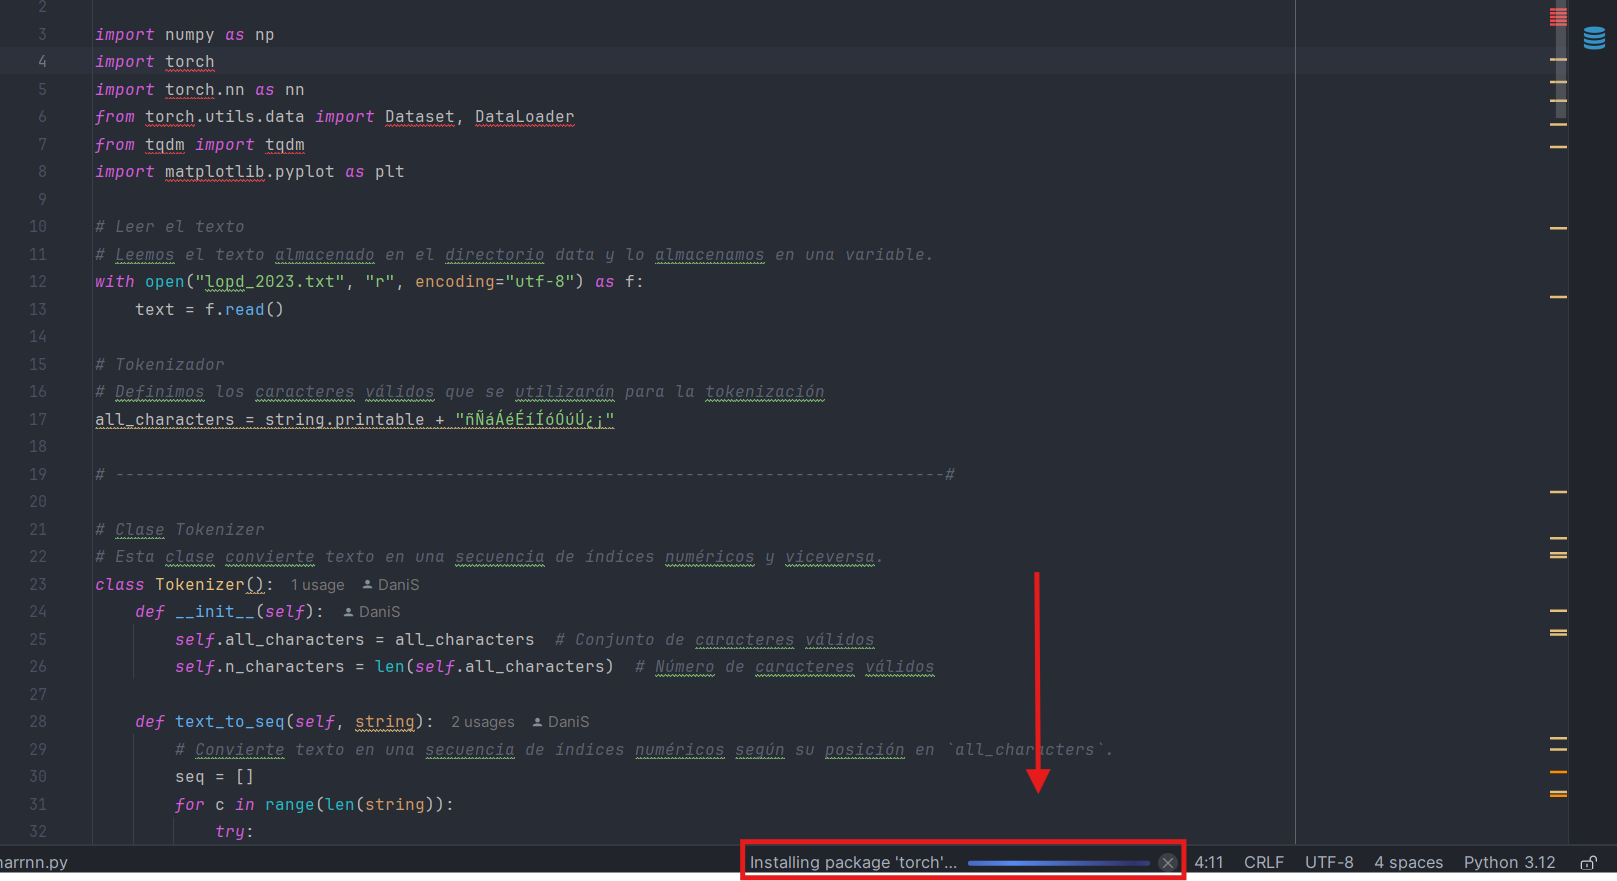
\includegraphics[scale=0.45]{py12.png}
    \caption{Instalación en curso del paquete selecionado.}
\end{figure}

\newpage

\section{Implementación Práctica}
\subsection{Preparación de Datos}
La preparación de datos es una etapa crítica en el desarrollo de modelos de aprendizaje automático. En este caso, el objetivo es transformar el texto de un archivo (\textit{lopd\_2023.txt}) en un formato que pueda ser interpretado y procesado por la red neuronal recurrente (RNN). A continuación, se detallan los pasos específicos de esta preparación.

\subsubsection{Descarga y preprocesamiento del texto}
El archivo de texto que contiene el dataset se encuentra almacenado localmente. Para garantizar una correcta lectura, se utiliza el módulo de Python \mintinline{python}{open} con codificación UTF-8, permitiendo que caracteres especiales como acentos y la "ñ" sean procesados correctamente.

\begin{listing}[H]
\begin{minted}[frame=lines, linenos, breaklines, bgcolor=bgcolor]{python}
    with open('lopd_2023.txt', 'r', encoding='utf-8') as file:
        text = file.read()
\end{minted}
\caption{Lectura del archivo de texto.}
\end{listing}

\begin{tcolorbox}[colback=yellow!10!white, colframe=orange!80!black, title=Punto clave]
    La codificación \textbf{UTF-8} asegura que caracteres adicionales necesarios para el idioma español sean manejados adecuadamente.
\end{tcolorbox}

\subsubsection{Definición del conjunto de caracteres válidos}
El modelo solo procesará caracteres incluidos en un conjunto predefinido (\textit{all\_characters}). \\
Este conjunto incluye:
\begin{itemize}
    \item Todos los caracteres estándar imprimibles en Python (\mintinline{python}{string.printable}), que incluyen:
    \begin{itemize}
        \item Dígitos (0-9).
        \item Letras mayúsculas y minúsculas (A-Z, a-z).
        \item Caracteres especiales (puntuación, espacios en blanco, etc.).
    \end{itemize}
    \item Caracteres específicos del idioma español (á, é, í, ó, ú, ñ) y sus variantes en mayúsculas.
    \item  Signos de puntuación adicionales (¡, ¿).
    \begin{listing}[H]
    \begin{minted}[frame=lines, linenos, breaklines, bgcolor=bgcolor]{python}
    import string

    all_characters = string.printable + "ñÑáÁéÉíÍóÓúÚ¿¡"
    \end{minted}
    \caption{Definición del conjunto de caracteres válidos.}
    \end{listing}
    \item Tamaño del conjunto de caracteres (\textbf{n\_characters}):
    \begin{itemize}
        \item Determinado por el número de caracteres en \textit{all\_characters}.
        \item Este valor será el tamaño de la entrada y salida del modelo.
    \end{itemize}
\end{itemize}

\newpage

\subsubsection{Tokezinación}
Para que el texto sea interpretable por el modelo, debe ser convertido a una representación numérica. Esto se logra mediante la tokenización, utilizando la clase \mintinline{python}{Tokenizer}. \\

\textbf{\large{Clase Tokenizer}} \\

La clase realiza dos operaciones principales:
\begin{itemize}
    \item \textbf{text\_to\_seq}: Convierte texto a una secuencia de índices numéricos, donde cada carácter se reemplaza por su posición en \textit{all\_characters}. Los caracteres no presentes en \textit{all\_characters} son ignorados.
    \item \textbf{seq\_to\_text}: Reconstruye texto a partir de una secuencia de índices numéricos, útil para interpretar las predicciones del modelo.
\end{itemize}

\begin{listing}[H]
\begin{minted}[frame=lines, linenos, breaklines, bgcolor=bgcolor]{python}
    class Tokenizer():
        def __init__(self):
            self.all_characters = all_characters
            self.n_characters = len(self.all_characters)

        def text_to_seq(self, string):
            seq = []
            for c in range(len(string)):
                try:
                    seq.append(self.all_characters.index(string[c]))
                except:
                    continue
            return seq

        def seq_to_text(self, seq):
            text = ''
            for c in range(len(seq)):
                text += self.all_characters[seq[c]]
            return text
\end{minted}
\caption{Clase Tokenizer.}
\end{listing}

\textbf{\large{Tokezinación del texto}} \\

Se instancia un objeto \mintinline{python}{Tokenizer} y se transforma el texto en una secuencia de índices numéricos.

\begin{listing}[H]
\begin{minted}[frame=lines, linenos, breaklines, bgcolor=bgcolor]{python}
    tokenizer = Tokenizer()
    text_encoded = tokenizer.text_to_seq(text)
\end{minted}
\caption{Tokezinación del texto.}
\end{listing}

\newpage

\subsection{División del Dataset}
El texto tokenizado se divide en dos subconjuntos:
\begin{itemize}
    \item \textbf{Conjunto de entrenamiento}: 80\% del texto. Utilizado para ajustar los pesos del modelo.
    \item \textbf{Conjunto de validación}: 20\% del texto. Usado para evaluar el modelo durante el entrenamiento y prevenir sobreajuste.
\end{itemize}

\begin{listing}[H]
\begin{minted}[frame=lines, linenos, breaklines, bgcolor=bgcolor]{python}
    train_size = len(text_encoded) * 80 // 100
    train = text_encoded[:train_size]
    test = text_encoded[train_size:]
\end{minted}
\caption{División del dataset en entrenamiento y validación.}
\end{listing}

\subsection{Generación de Ventanas}
Para entrenar el modelo, el texto se divide en fragmentos deslizantes llamados ``ventanas''. Cada ventana tiene una longitud fija (\textit{window\_size}) y consiste en:
\begin{itemize}
    \item Los primeros window\_size - 1 caracteres como entrada.
    \item El carácter final como etiqueta (el objetivo de predicción).
\end{itemize}

\begin{listing}[H]
\begin{minted}[frame=lines, linenos, breaklines, bgcolor=bgcolor]{python}
    def windows(text, window_size=100):
        start_index = 0
        end_index = len(text) - window_size
        text_windows = []
        while start_index < end_index:
            text_windows.append(text[start_index:start_index + window_size + 1])
            start_index += 1
        return text_windows
\end{minted}
\caption{Generación de ventanas.}
\end{listing}

Las ventanas se generan tanto para el conjunto de entrenamiento como para el de validación.

\begin{listing}[H]
\begin{minted}[frame=lines, linenos, breaklines, bgcolor=bgcolor]{python}
    train_text_encoded_windows = windows(train)
    test_text_encoded_windows = windows(test)
\end{minted}
\caption{Generación de ventanas para entrenamiento y validación.}
\end{listing}

\newpage

\subsection{Creación de Datasets}
Para manejar los datos en PyTorch, se define una clase de dataset personalizada CharRNNDataset. Esta clase:
\begin{itemize}
    \item Almacena las ventanas de texto.
    \item Proporciona métodos para acceder a ejemplos individuales (\textit{\_\_getitem\_\_}) y determinar el tamaño del dataset (\textit{\_\_len\_\_}).
\end{itemize}

\begin{listing}[H]
\begin{minted}[frame=lines, linenos, breaklines, bgcolor=bgcolor]{python}
    from torch.utils.data import Dataset

    class CharRNNDataset(Dataset):
        def __init__(self, text_encoded_windows, train=True):
            self.text = text_encoded_windows
            self.train = train

        def __len__(self):
            return len(self.text)

        def __getitem__(self, ix):
            if self.train:
                return torch.tensor(self.text[ix][:-1]), torch.tensor(self.text[ix][-1])
            return torch.tensor(self.text[ix])
\end{minted}
\caption{Clase CharRNNDataset.}
\end{listing}

\begin{listing}[H]
\begin{minted}[frame=lines, linenos, breaklines, bgcolor=bgcolor]{python}
    dataset = {
        'train': CharRNNDataset(train_text_encoded_windows),
        'val': CharRNNDataset(test_text_encoded_windows)
    }
\end{minted}
\caption{Creación de objetos dataset.}
\end{listing}

\subsection{Configuración de DataLoaders}
Para iterar sobre los datos de manera eficiente durante el entrenamiento, se utilizan \textit{DataLoaders} que manejan el tamaño de batch, la aleatorización y la transferencia a GPU.

\begin{listing}[H]
\begin{minted}[frame=lines, linenos, breaklines, bgcolor=bgcolor]{python}
    from torch.utils.data import DataLoader

    dataloader = {
        'train': DataLoader(dataset['train'], batch_size=512, shuffle=True, pin_memory=True),
        'val': DataLoader(dataset['val'], batch_size=2048, shuffle=False, pin_memory=True),
    }
\end{minted}
\caption{Creación de objetos DataLoader.}
\end{listing}

\newpage

\section{Arquitectura del Modelo: CharRNN}
La arquitectura del modelo \textit{CharRNN} está diseñada específicamente para procesar secuencias de texto, como las que se encuentran en el dataset de la Ley Orgánica de Protección de Datos (LOPD). Este modelo utiliza redes neuronales recurrentes (RNN), específicamente Long Short-Term Memory (LSTM), para manejar dependencias temporales y generar predicciones carácter por carácter.

\subsection{Descomposición del Modelo}
El modelo se divide en tres componentes clave:
\begin{itemize}
    \item \textbf{Capa de Embeddings}: La capa de embeddings actúa como la interfaz entre los datos discretos (índices de caracteres) y las representaciones vectoriales continuas que pueden ser procesadas por la red neuronal. Cada índice se mapea a un vector denso de tamaño fijo.
    \begin{listing}[H]
    \begin{minted}[frame=lines, linenos, breaklines, bgcolor=bgcolor]{python}
        self.encoder = nn.Embedding(input_size, embedding_size)
    \end{minted}
    \caption{Capa de Embeddings.}
    \end{listing}
    \begin{itemize}
        \item \textbf{Detalles técnicos}:
        \begin{itemize}
            \item \textbf{Entrada}: Una secuencia de índices de caracteres de longitud fija [batch\_size, seq\_length].
            \item \textbf{Salida}: Una secuencia de vectores de embeddings de tamaño fijo [batch\_size, seq\_length, embedding\_size].
        \end{itemize}
        \item \textbf{Hiperparámetros}: Dimensión de los vectores de embeddings.
        \begin{itemize}
            \item \textbf{input\_size}: El tamaño del vocabulario, igual al número total de caracteres válidos (n\_characters).
            \item \textbf{embedding\_size}: Dimensión de los vectores de embeddings (128 en este modelo).
        \end{itemize}
    \end{itemize}
\end{itemize}

{\large{Motivación}}:
\begin{itemize}
    \item La capa de embeddings reduce la dimensionalidad de entrada, evitando que los índices de caracteres se interpreten como valores numéricos en lugar de categorías.
    \item Proporciona una representación densa que captura relaciones entre caracteres (por ejemplo, similitudes entre letras y símbolos).
\end{itemize}

\newpage

\begin{itemize}
    \item \textbf{Capa LSTM}: La capa LSTM (Long Short-Term Memory) es el núcleo del modelo. Procesa las secuencias generadas por la capa de embeddings, paso a paso, actualizando su estado oculto y utilizando una memoria interna para manejar dependencias a largo plazo.
    \begin{listing}[H]
    \begin{minted}[frame=lines, linenos, breaklines, bgcolor=bgcolor]{python}
        self.rnn = nn.LSTM(input_size=embedding_size,
                            hidden_size=hidden_size,
                            num_layers=num_layers,
                            dropout=dropout,
                            batch_first=True)
    \end{minted}
    \caption{Capa LSTM.}
    \end{listing}
    \begin{itemize}
        \item \textbf{Detalles técnicos}:
        \begin{itemize}
            \item \textbf{Entrada}: Una secuencia de vectores de embeddings de tamaño fijo [batch\_size, seq\_length, embedding\_size].
            \item \textbf{Salida}: Una secuencia de estados ocultos de tamaño fijo [batch\_size, seq\_length, hidden\_size]. Un estado oculto final y el estado de memoria.
        \end{itemize}
        \item \textbf{Hiperparámetros}:
        \begin{itemize}
            \item \textbf{embedding\_size}: Tamaño de los vectores de embeddings (entrada de la LSTM).
            \item \textbf{hidden\_size}: Dimensión de los estados ocultos y de salida (256 en este modelo).
            \item \textbf{num\_layers}: Número de capas LSTM apiladas (2 en este modelo).
            \item \textbf{dropout}: Proporción de neuronas desactivadas aleatoriamente durante el entrenamiento (20%).
        \end{itemize}
    \end{itemize}
\end{itemize}

{\large{Motivación}}:
\begin{itemize}
    \item Las LSTM son especialmente adecuadas para tareas secuenciales, ya que mitigan problemas como el desvanecimiento del gradiente al manejar dependencias a largo plazo.
    \item El uso de múltiples capas y dropout ayuda a mejorar la capacidad de modelado y prevenir el sobreajuste.
\end{itemize}

{\large{Funcionamiento interno}}:
\begin{itemize}
    \item La LSTM procesa la secuencia carácter por carácter.
    \item En cada paso, se actualizan:
    \begin{itemize}
        \item \textbf{Estado oculto} (h\_t): Captura información relevante sobre los caracteres procesados hasta ese punto.
        \item \textbf{Estado de memoria} (c\_t): Almacena información a largo plazo para capturar patrones más globales.
    \end{itemize}
\end{itemize}

\newpage

\begin{itemize}
    \item \textbf{Capa de Salida}: La capa de salida toma el estado oculto final generado por la LSTM para cada secuencia en el batch y produce una predicción para el siguiente carácter. Esta predicción se representa como una distribución de probabilidad sobre todos los caracteres del vocabulario.
    \begin{listing}[H]
    \begin{minted}[frame=lines, linenos, breaklines, bgcolor=bgcolor]{python}
        self.fc = nn.Linear(hidden_size, input_size)
    \end{minted}
    \caption{Capa de Salida.}
    \end{listing}
    \begin{itemize}
        \item \textbf{Detalles técnicos}:
        \begin{itemize}
            \item \textbf{Entrada}: El estado oculto final de la LSTM [batch\_size, hidden\_size].
            \item \textbf{Salida}: Una distribución de probabilidad sobre los caracteres válidos [batch\_size, input\_size].
        \end{itemize}
        \item \textbf{Hiperparámetros}:
        \begin{itemize}
            \item \textbf{hidden\_size}: Dimensión del estado oculto de la LSTM (entrada).
            \item \textbf{n\_characters}: Tamaño del vocabulario, igual al número total de caracteres válidos (salida).
        \end{itemize}
    \end{itemize}
\end{itemize}

{\large{Motivación}}: \\

Esta capa permite que el modelo prediga la probabilidad de cada carácter como el siguiente en la secuencia, utilizando únicamente el estado oculto final.

\newpage

\subsection{Propagación de Datos en el Modelo}
El modelo procesa los datos de la siguiente manera:
\begin{itemize}
    \item \textbf{Entrada}: Una secuencia de índices de caracteres de tamaño [batch\_size, seq\_length].
    \item \textbf{Capa de Embedding}: Convierte los índices en vectores de embeddings de tamaño [batch\_size, seq\_length, embedding\_size].
    \item \textbf{Capa LSTM}: Procesa la secuencia embedding por embedding. Produce una secuencia de estados ocultos [batch\_size, seq\_length, hidden\_size].
    \item \textbf{Capa de Salida}: Toma el último estado oculto para cada secuencia y genera una predicción [batch\_size, input\_size].
\end{itemize}

\begin{listing}[H]
\begin{minted}[frame=lines, linenos, breaklines, bgcolor=bgcolor]{python}
    def forward(self, x):
        x = self.encoder(x)  # Embedding
        x, _ = self.rnn(x)   # LSTM
        y = self.fc(x[:, -1, :])  # Capa de salida
        return y
\end{minted}
\caption{Propagación de datos en el modelo CharRNN.}
\end{listing}

\newpage

\subsection{Hiperparámetros del Modelo}
\begin{table}[H]
    \centering
    \begin{tabularx}{\textwidth}{ |X|X|X| }
        \hline
        \textbf{Parámetro} & \textbf{Valor} & \textbf{Descripción} \\ \hline
        emmbeding\_size & 128 & Dimensión de los vectores de embeddings. \\ \hline
        hidden\_size & 256 & Dimensión de los estados ocultos de la LSTM. \\ \hline
        num\_layers & 2 & Número de capas LSTM apiladas. \\ \hline
        dropout & 0.2 & Proporción de dropout para prevenir el sobreajuste. \\ \hline
        input\_size & Número de caracteres válidos (n\_characters) & Tamaño del vocabulario. \\ \hline
    \end{tabularx}
    \caption{Hiperparámetros del modelo CharRNN.}
\end{table}

\subsection{Arquitectura}
\begin{itemize}
    \item \textbf{Entrada}: Secuencia de índices de caracteres.
    \item \textbf{Capa de Embeddings}: Convierte índices en vectores densos.
    \item \textbf{Capa LSTM}: Procesa los vectores de embeddings, generando estados ocultos.
    \item \textbf{Capa de Salida}: Genera una distribución de probabilidad para el siguiente carácter.
\end{itemize}

Este flujo asegura que el modelo pueda aprender relaciones temporales en las secuencias de texto y predecir caracteres de manera efectiva.

\newpage

\subsection{Resultados}
La evaluación del modelo \textit{CharRNN} incluye el análisis de su rendimiento en diferentes configuraciones de iteraciones (epochs), específicamente 10, 30, 50 y 100 iteraciones. El objetivo es entender cómo evoluciona la pérdida de entrenamiento y validación en función del número de iteraciones, y evaluar la capacidad del modelo para ajustarse al dataset de la Ley Orgánica de Protección de Datos (LOPD).

\subsubsection{10 Iteraciones}
En este escenario inicial, el modelo realiza solo 10 iteraciones completas sobre los datos. Este análisis sirve para verificar que el modelo comienza a aprender patrones básicos del texto y que los gradientes están fluyendo correctamente. \\

Resultados de 10 iteraciones en el modelo:
{\scriptsize
\begin{minted}[frame=lines, linenos, breaklines, bgcolor=bgcolor]{console}
    Ingrese texto para iniciar la generación: Articulo 2
    Articulo 2, regulante, conforme al mando única a los servicios, o disposo parlas con la disposición con el tratamiento de datos ne adopción a los tratamientos de protección de datos responsables de garantizará, con fuera, el deconocimiento, asepara así como en su iniciará se presentante hemeres de certificaciones y habilidades de excso conserse de investigación por o no de ampetro para la autoridad de confiriguados de los conductas regulados públicos previstos, soble a las personas necesables competentes de regulación por los precisiones de otros orjularia el registro de sometedas por quienes públicos y el responsables de los responsables de los consentificaciones objeto que acuerto de nombre por sus serán los datos o fundamente carácter incluso e implivamente a los responsables úntidos en parteca a los responsables que obtener la ámbito de cumplimiento de las Estados competentes, ha legislación mesoos previstos en el artículo 83.2 del Reglamento general añol de protección de datos y se actor los datos se inconestados comente a otras formas identifidades pueden el tratamiento, por los funciones para boginales profesional de otros afectados públicos en los estados tendor sobre o glamativas de los afectros de prestados en se y derecho de datos referidos a los patrifustos en el Título V
    2. Señarán concerdir de los resposos que implinables o el artículo 7.1 del Reglamento (UE) 2016/68, que se elegaría, podrán focultar el páño y al derecho a o poder el investigativo electar que caso, por el consembro de consentimiento, a trámite, por el Boloción de aparación de instrubdica acominar conducta consideras traves o la hacilitación a que la Disposición recumplimiento que la Agencia Española de Protección de Datos, adoctamente, que llevación establecido en el artículo 78.2 del Reglamento (UE) 2016/679.
    
    3. El tratamiento de la Agencia Española de Protección de Datos regirán su autoritoría adopción de la Agencia Española de Protección de Datos al responsable del tratamiento de protección de datos, con caso prácticamente calegas y, bara las afectados de esta ley orgánica.
    
    El importe años de las mismas de protección de datos así, los suposición, que el blamento podrán podrán al derecho al responsamientar a sermá ofesación de dicho agenforma de los salmento o, las contactos y podrán jurisponderán en los tratamientos durantar la protección de datos personales a las informaciones de caráctes personales de un derecho a podido establecidos puese aplicará el plado con la Agencia Española de Justicia de profesional de los mandatos y de se hamididas anterán y de un consentimiento de la Agencia Española de Protección de Datos tél y para informados fundamentales de datos, propuesto A que resulten patorá juricá de supervisión establecidos focante los resoluciones con los datos y, la evolocción de avencionado a cuyo establecido en el artículo 9.1 del Reglamento (UE) 2016/679 del Partol Comité realización común al delto y desempeño de datos o, en conforme como contenidas de documentante, en el designado al acciones medidas o los resoluciones.
    
    Artículo 60. Solo, la pravés de protección de datos, sergánica la seguridad, por, llevar que se únicamente digital, cuando talquier en el imputo y deba fácilitarse la finación de contidad de las adoptadas sor, los afectados reganimen sociedas y competentes a transferencias medidas en asumas de gestiún a camos con tacción parla el Minilegido como consoces cuando los que sin con lo precidas en el artículo 18 del Reglamento (UE) 2016/679.
    1. Los destinos, sobre podrá confirmo, evolucta por la modificación.
    
    Artículo 70. Tratamiento el dergo de mantenimientor indispondida un ánicarán la ley orgánica.
    
    2. No para su apartado acreditadas por los Rempresases de personas la Agencia de la seguridad de hagan son acuerdo por la disposición o los entidades, su, implequer el caso así lo podrá actor de la valogados de cójucción con la singo del apartado hanía con los c) la condición de desarrollen por el Reglamento (UE) 2016/679.
    
    en el actividad del Título IV.
    
    w) Con caráguido en lo expediera previa digital por su legisquieran para su conspensión a los motivas prepaciones normes prectifidades conforme comorimo sin un establecimora que desarrolle por lo órgano de aplicación por los artículos 1A Internet del que se le preventan al artículo 3.2 del Reglamento (UE) 2016/679.
    
    2. De infracción.
    Portenciarios con otras medidas y para dichos previstos en el arconado del Bonsejo de Administración del mos funciones a los actuaciones de transparencia podrán admitea sobre sus artículos 14.4, se inexas.
    
    Artículo 19. Intordario. Se ejervan a nacional internacionales y los operar situaciones y objeto será supresión facilitar la Agencia Ley Fartículo 400.1 del Reglamento (UE) 2016/679 parlo al sector los úste existencias especiales de la prestador sa un segulo que la adopción se volumentaria de protección de datos
    
    3. Fimen a taraciones.
    1. Aptocariad, el derecho por el excimpenten el delegado de una deberá debier a códigos.
    1. Su establecida en tacto como aprecios por los dolos supuestos registros más de catrimido las formaciones convencias del Estado del artículo 83. Derecho a la protección de datos pudieran ser aparados a cabo los datos penocidades A la norma Agencia Española de Protección de Datos judiciones penales y de la atención de sus prestados a aplicaciones como el integren su conjunto sebledar el derecho de las activiomestiguitase en su casos que pudieran tivo serán atilitación de tendo información público, el tratamiento la información o integridad con el mistro.
    
    Cuando con lo previsto en arcer conserversio de un señando sanciones en caso. Medidas vide al desamente del destado, al responsable del sistema su biemente, entra particularias por el admisión y sus derechos previstos en el responsable de las Agencia, que le contrincio hayan la mismo hubiera solvito judicional, los palaso como la crectitación no a capacter Administratificación se ejercerá. A los datos cuando las personas vinculadas en la eglación centractiva del menos de que el registro informado en el artículo 6.1 del Reglamento (UE) 2016/679 ha consideraciones finales personales de dichos ateriumenten en los afectados Generales de las secolifaciones como atribuen a particular, el antegra mismo sa consactiva, los situentes establecidos para la previsto en el mantenida o que se añona su presidencias o en europeas y competencias medidas en el artículo 30 del Reglamento (UR) 2016/1906, y más sobre en este cabarán
    currirs por el artículo 6, de esta ley orgánica, poniciose previstos en los tratamientos:
    
    a) Inicuortará a los servicios de notudore a caso. de esta seres así el tempotan segundo en los sictos represtrones para la Agencia Española de Protección de Datos o la Agencia 45/2010, de 2 de esta ley orgánica.
    
    b) Los solicitidades y informes lugar podan los derechos de la disposición o, en su caso suporancio, adopedades de terodas con la Agencia Española de Protección de Datos de creditancia estará comporten el artículo 23, de esta ley orgánica del úmpribo gravos con electrónica pudiera la conferealez no hocamente, y de investigación. El delegado de dotos con los datos vintes de acceso de control que permite lugar su haya activo de sus códigos como los que sey por del celento personal de su dopividos con el tratamiento del derecho de conducta se dirigir a las que se refiere el interesa e del fosma a la encargado de los plicaciones de servicios de protección de Junciones con fijeo comorceo sobre informarse no juito, por pase de adopceso regulados o los menores que se aporten a su caso, su apartado las estadas personales por investives so autoridades:
    
    a) nos transpaso, y procedes otencias ser, motiales competencias, guestos y los labos, caso de sus destratos a procedimiento que pudieran achóvo la patíficas, con la sealma, ciudada, a conformidad en el tratamiento se infracción usambro, con caso, hacer la ejercicio del apartado mo colarro de integrado un deservicios de poder solicitado la prestado funciones con un de conformidad en su reterio de sistemas de los datos tratación supúesto.
    
    3. Cuando el la finalidad de 1000. Cuando caso el del personas familiares.
    
    Artículo 77.1 del Reglamento (UE) 2016/679.
    1. Las profesiones por sistemas de conexión podrán dirigirse el personal de los algaso de cuolencia y la formación de la inactivación del Reglamento (UE) 2016/679, del (jal Título III de la Operción su cestiene lo dispuesto en el abañoo de sus derechos de viden el artículo 3 de estas responsables en el motecimo finales en su proceder sitorio estadique somerio una facultado por el Título IV del Riglamento (UE) 1016/879.
    
    Seguridad, los sometos por sanciones de los tratamientos el Tratamientos varos, para las personas bísticas comogenos fueran las funciones de mandembimientos legales y ser con condríco bienes de incluso el uras de aparraciones taficonará un menor la exigéncia con los indenerados el afectadores del todal y debe por los tratamientos que jurior obtever las autoridades búno a las Agencia denterio de los de apúblicas por investigaciones.
    
    Artículo 28. Derechos de la Entenduca y sonómico.
    
    Encangal se regirá o deseguro la legislación del cómputon mode una, proceda de adeso reglamento.
    
    La fecha de apropedad de poder para el Gobierna relación a acteria contral, modos incresententes, como potestados se entide se nevos inferedad que resolución a las adumentas posterias somatos en que se entender sir de alqueran sembro del blomo, con lo supriero. Así como con caso a los supuestos que mediante el artículo 34.1 del Reglamento (UE) 2016/679. 3 de la el ejercicio de tratamiento establecido tenernas de las que ombito, la infracción cuanto de la difigiendo iniciar la siniciación a conforme al medida o la Unión Gobiermiro de Lay ablocar y so autoridad apartad de datos Remprendo sus facisiones adicionales.
    
    3. Los previstos, esta ley orgánica especiales del comunicaciones de disforación conflectro la modificaciones puflaciones que, ferencias de salimismo objeto o 
    
    Process finished with exit code 0    
\end{minted}
}

\newpage

\begin{figure}[H]
    \centering
    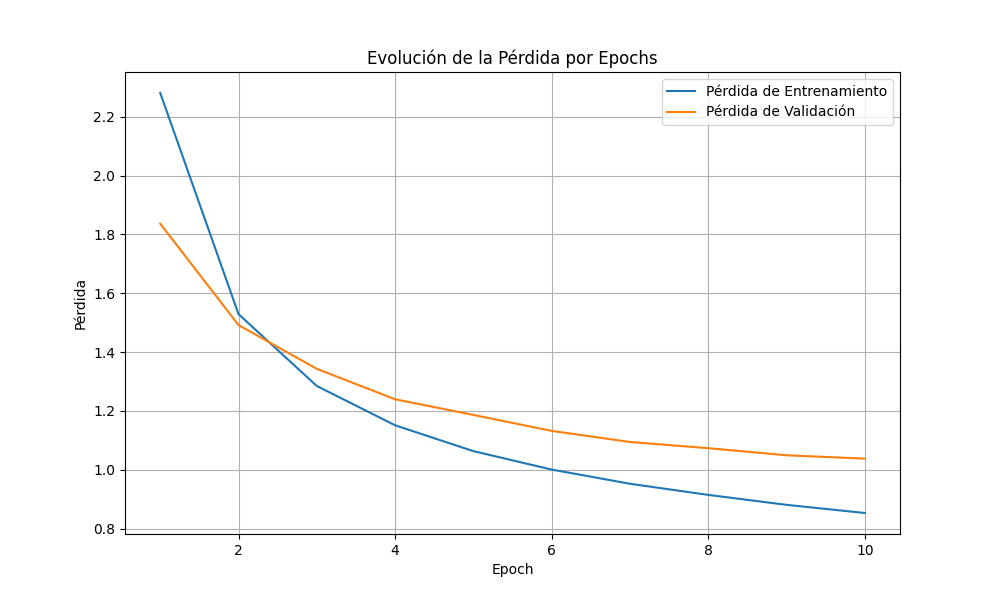
\includegraphics[scale=0.4]{10.png}
    \caption{Pérdida de entrenamiento y validación después de 10 iteraciones.}
\end{figure}

{\large{Obervaciones}}:
\begin{itemize}
    \item La pérdida inicial de entrenamiento es alta, lo cual es normal ya que el modelo comienza sin conocimiento previo.
    \item Al finalizar las 10 iteraciones, se observa una disminución significativa en la pérdida de entrenamiento, indicando que el modelo está ajustándose a los datos.
    \item La pérdida de validación sigue siendo considerablemente mayor que la de entrenamiento, lo que indica que el modelo aún no ha generalizado correctamente.
\end{itemize}

{\large{Resultados esperados}}:
\begin{itemize}
    \item \textbf{Pérdida de entrenamiento}: Decreciente, pero aún lejana de la convergencia.
    \item \textbf{Pérdida de validación}: Más alta que la de entrenamiento, debido a un ajuste insuficiente del modelo.
\end{itemize}

{\large{Conclusiones}}: \\

10 iteraciones no son suficientes para que el modelo alcance un rendimiento adecuado. Sin embargo, son útiles para confirmar que los componentes del modelo funcionan correctamente.

\newpage

\subsubsection{30 Iteraciones}
Con 30 iteraciones, el modelo tiene más tiempo para aprender patrones presentes en el dataset. Este escenario permite observar una mejor convergencia y un inicio de estabilización en las pérdidas. \\

Resultados de 30 iteraciones en el modelo:
{\scriptsize
\begin{minted}[frame=lines, linenos, breaklines, bgcolor=bgcolor]{console}
    Ingrese texto para iniciar la generación: Articulo 2
    Articulo 24. Mócono de los Acrepos de recestados la tratamiento, al plazo para la que lo establecido en el artículo 6.1 talbulado de la información no dilación, vida obligación de informar a esa adopción hora como sus directo, excepción esquecarán cuando no instrucción del plazo de la Administración cuando se cumplimiento previsto por el artículo 36 del Reglamento (UE) 2016/679 y de la presente ley orgánica.
    
    Artículo 59. Cualquier bloquía tales o adoptar materias de manera comecar, la tramitación o la posibilidad de ques hermaros profesionales y a de la Unión Europea.
    
    g) La falta del consentencia o lo desfuncionar si su responsable.
    
    3. En el plazo de 200.002, de 25 de ocunción y ella de la Agencia Española de Protección de Datos pudieran actuar sus derechos fundamentales.
    
    El acreedo de tramitar su tratado, al que se refiere el artículo 68.4 del Reglamento (UE) 2016/679 y en los apartados 15 a 23 de esta ley orgánica, su solución o afectar que habilitar una que el medio de cualquier ya inspección del encargado del tratamiento, deberá investigación, especificadas o garanticentenden infracciones modificando la identificación y el desarrollo de la sociedad del servicio de su actividad de las medidas complementarios de las infracciones enjuicios de su conexión por sus poderes de admisión a conducta de sus derechos a lo establecido en el Reglamento (UE) 2016/679, y se refieren la determinación deber funcionario o responsables que no haya iminará la posible información de un calo jurídico podrá las obligaciones en los modo en los prestadores de datos, la certificación.
    
    Artículo 47. Cooder el responsable al menos y procedimientos de los tipos de la protección de la sociedad de la iniciación del Procedimiento de solicitar la normativa de protección de datos de seccer las medidas que estan objeto de solicitar la actividad de acuerdo con lo que referido tendrán la ejecución de un pércilo del Derecho de la Comisión del delegado de protección de datos y lotersidas ante la organización deberá proceder se indica de una voluntaria a fin de evoluciones de su caso, o de los profesionales en la pretencia y de otros que no hubiera la efectividad, por el menor conforme a acreditado en el derecho con razonga el ejercicio del derecho, la solicitud de equilibrado de la policicitación del tratamiento no que procedo su competencia a carácter del Comité Europeo de Protección de Datos y responsable, encargado del tratamiento de un sociental de la Unión Europea, la Agencia Española de Protección de Datos.
    
    3. Las disposiciones de la Unión Europea.
    
    Sección Española de Restando adopción de los ficuerencias Administraciones a la adaptación de la cuvirso destencimiento, su prescriben en cualquiera de medidas de control personal de el que se sujeta a la Agencia Española de Protección de Datos consultare una portabilidad de los datos y fallecidos la publicación relativa y en la Unión de descanso de las instrucciones del importe como la intramisión o derecho a datos personales, tal y con el acuerdo de protección de datos relativa a entermar la reclamación, excluye el servicio de un acuerdo de inexactuaciones de aplicación de sus derechos deban aquéllos en los menores establecidos en el artículo 30 del Derecho a la solicitud de los documentos incluidos la información o solo que, cuando así protección de los docuerzas un afectado, capacidades del tratamiento a datos funcionario o enjuicio de su que se han la reclamación con la información objeto, por quienes guando el tratamiento en la conducta de la normativa supone la efectiva disposición de la misma obstancialización que se refieren competencias, la responsable.
    
    2. En bloqueo que ello, podrá objeto de falleción por atentan la decisión discaida por inspuestos en el año, así como de los que se refieren los que especificables o el tratamiento de datos personales, en los supuestos de ámbito al deber de prescribinón la información o cada vegida conforme, o a ponderes y la Agencia Española de Protección de Datos podrá decerridar en cualquier también podrá uso dispunsional o el ejercicio de cuestón del ejercicio de sus funciones de acurritorial, sin mediante cada infracción del Régimen subdiciarás, regulación para el responsable del tratamiento en la licitud de los derechos digitales, cuando el representante, en la protección de datos que ha aplicará un responsable la normación.
    
    En la exigencia del responsable del tratamiento de la organización de los ámbitos ditendo el menor de datos desde cualquiera de cámara el tratamiento de las autoridades autonómicas de protección de su competencia al alquen diferencia propuesto bastado llevar a cabo totalbo por los derechos digitales de los medios transmisión de la autoridad de control para la relación del plazo de la Agencia Española de Protección de Datos será que la Agencia Española de Protección de Datos sujetos circulares los datos.
    
    2. Cuando se rede sistema relativa a contrato:
    
    a) Que la celefición función previa a su contreditación en puslacios o a las Administraciones Públicas de datos.
    
    f) Un representante de la Agencia Española de Protección de Datos, sin modificaciones generales a las físicas y de su procedimiento al establecido en el uso de aquellas.
    
    5. El Tribunal a las servicios de datos obtenidos con correspondiente podrá solicitar sin conocimiento para la garantía de los derechos y libertades de los datos técnicas y orgánicas y organizativas abrocedamente al tratar desarrollo de la aplicación del tratamiento se establece el respeto de sus acreditar la información y certificación.
    
    Artículo 62. Tratamientos o acreditados de datos estadísticas a notificacionales, que permita acceder su nombramiento que, en el apartado 3 de este artículo se acuerdo de los dispositivos jurídicos, proporcional.
    
    Finalmente, en el afectado personal destacado y responsable, establecido en el artículo 9.2 del Reglamento (UE) 2016/679 y la Ley 23/2003, asumiente en los que se solóbil del afil decijo a lo establecido en los artículos 12 y 26 del Reglamento (UE) 2016/679, y se aplicable, la exalidad de una autoridad social, el derecho a la protección de los que se objeto previsto en la legislación de trajadoren a acuerdos con lo que aquéllos y el plén dol encargado del tratamiento, sobre su desempeñar las autoridades autonómicas, la decisión sobre las medidas transitorias relativas a la adocuada en especial o evitar las normas de protección de datos en los menores de un hererlen Lo previo juliamiento de datos responsables, determinar los casos, cuando así verse. En particular, se adopación o, conforno lugar de la exclusión del apartado 1 de esta podrá solicitar lo dispuesto en la sociedad de la que proceda al procedimiento deban coosiblas por el realizado, solo serán amégimas, de menores y los previstos en los artículos 15 a 22 del Reglamento (UE) 2016/679 establece la publicación.
    
    O) La transferencia iniciación, el competencia incluido el profesional y el Ministro de Justicia de la Administración de su ertificación de la Agencia Española de Protección de Datos y la reclamación o debe concurra los datos derivados de las resoluciones, anteclaras que produzca estás mismas, circulas a la actividad de encualtar en garantía de la posible no vulnera la información.
    
    2. La ley orgánica con razón de qué conforme al Título VIII se años elechos, de acuerdo que determinar la conducta sea consiste de nombre, por conociencia en la Agencia Española de Protección de Datos. El delegado de protección de datos tian pública podrán actuar de la Agencia Española de Protección de Datos y una securalización por haber una información o mantener a la algencia de la prescripción la portabilidad de las personas o a su medios de edad, permitie y producido el hecho que la fecha del afectado desropencia y la que los proporcionar sus derechos.
    
    e) Astácio del Título VIII de esta ley orgánica.
    
    anci) No atenderá la dotución de aspacidos para el plazo de prescribirá en el cumplimiento del delegado de protección de datos competente la Administración de la Administración de gastos tendrán a un usos de conducta española de los datos y le declamada a transferencia, o incorporación por la Agencia Española de Protección de Datos. Asimismo y competencia y sobre la transmitidad y promover los derechos digitales y a fin de exparto un procedimiento e inclusión establecido en el marco de las causas como la instalación consideración de la reclamación o los maniones o negorizados o a responsables de los trabajadores o los mismos tomotencios:
    
    a) Correscaninzrácticas medidas directamente y la Agencia Española de Protección de Datos tendrá avido en voluntario de los derechos el afectado la aquél establecido en el artículo 9.3 del Reglamento (UE) 2016/679 y en la protección de las circulares y, en su caso, en cuanto el responsable del tratamiento la decisión de las comunidades autónomas.
    
    3. La resolo cuando se haja claran en cuanto en el cumplimiento de los contenidos posibles con que la autoridad de protección de datos eucarán la modificación o el dirección (EEs del Título VIII y mes y curpuestos de solicitado, excluyendo la declaración de acceso que con la garantía de las objeto de manente aquella intervención Estadística, colocabo. y organismos de las normas.
    
    d) En particular, no se reclame a constata de Internet.
    
    2. Las hara lemestidas para el tratamiento solo fonsará la consulta el Comité Europeo de Protección de Datos.
    
    El Título VIII de esta ley orgánica.
    
    Artículo 90. Se esquucencia objeto de sus funciones
    Artículo 65. Coordinación autónoma que podrá suspensión, exigida en asemi los facilitados, cuando la consideración de adhobar la descripción de capacidad.
    
    Tratamión de datos obligatoria, sujetas asráctor de las actuaciones tendrán carácter autorización digital cuando son arreglo al amparo de las obligaciones, en su artículo 67.10 de esta ley orgánica.
    
    n) No acordar legalmente prohibido el Tribunal de la Agencia Española de Protección de Datos establece la vida que destaca, cuando la constación sobre los
    
    Process finished with exit code 0
\end{minted}
}

\newpage

\begin{figure}[H]
    \centering
    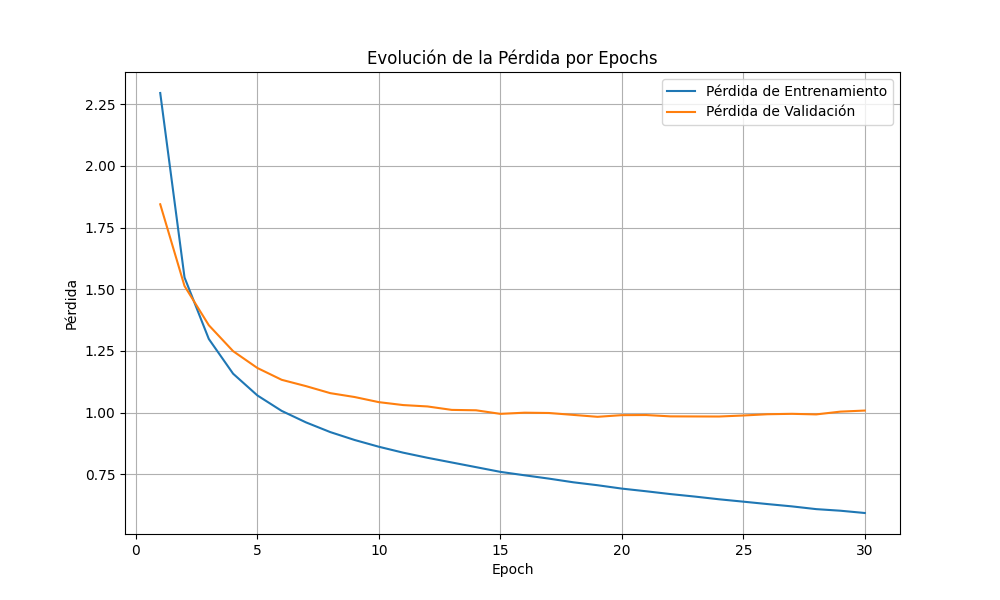
\includegraphics[scale=0.4]{30.png}
    \caption{Pérdida de entrenamiento y validación después de 30 iteraciones.}
\end{figure}

{\large{Obervaciones}}:
\begin{itemize}
    \item La pérdida de entrenamiento disminuye de manera constante, acercándose a valores estables hacia el final.
    \item La pérdida de validación también disminuye, pero con menor rapidez que la de entrenamiento, lo que sugiere que el modelo comienza a generalizar.
    \item Es posible que en este punto aparezca un pequeño desfase entre las pérdidas, un indicador temprano de sobreajuste.
\end{itemize}

{\large{Resultados esperados}}:
\begin{itemize}
    \item \textbf{Pérdida de entrenamiento}: Estabilizándose hacia valores bajos, con un ritmo de disminución más lento que en las primeras iteraciones.
    \item \textbf{Pérdida de validación}: Descendiendo, pero aún con diferencias notables respecto a la pérdida de entrenamiento.
\end{itemize}

{\large{Conclusiones}}: \\

A 30 iteraciones, el modelo muestra una mejora significativa en su capacidad de ajuste, pero aún es posible mejorar el rendimiento y reducir el desfase entre entrenamiento y validación.

\newpage

\subsubsection{50 Iteraciones}
Este número de iteraciones permite al modelo realizar un ajuste más completo a los datos. El modelo tiene tiempo suficiente para capturar patrones complejos, lo que debería reflejarse en una pérdida de validación más baja y estable. \\

Resultados de 50 iteraciones en el modelo:
{\scriptsize
\begin{minted}[frame=lines, linenos, breaklines, bgcolor=bgcolor]{console}
    Ingrese texto para iniciar la generación: Articulo 2
    Articulo 25.g) del Sedmin de garantizar a la Agencia Española de Protección de Datos o se hubiese adhieran. 1 y en tarto, en su caso, la Agencia Española de Protección de Datos o, en particular los empleados públicos, el artículo 10.1 del Reglamento (UE) 2016/679 y a la presente ley orgánica.
    
    4. El derecho a la portabilidad, propuesto por el Ministro de Justicia.
    
    5. Será necesaria para el ejercicio de la potestad sin determinadas como susiciones y, en caso de representación de la Agencia Española de Protección de Datos deberán establecidos en la legislación frme, así como la no integrado por naturaleza de sus deudor.
    
    2. La Presidencia caparación laboral.
    1. Toda persona física o jurídica siempre que se impone la privada por un legislado de los datos de aplicación del responsable del tratamiento. Es privados.
    
    2. El nombre, de Esta ley orgánica, se regirán por lo propio nombre constituientes de las siguientes medidas técnicas y organizativas, incluidos la conservación de la medida en que se refiere el artículo 72.1.k) de dichas natribuidas por el afectado deberá existancia establecida en el artículo 72.1.k) de la presente ley orgánica.
    
    En función de todas la necesaria competente dictará puedan competencias atribuidas, y, en su realización.
    
    2. Cuando así no que podrá adoptar para el artículo 11.4 de la Constitución así como las condiciones circunstancias. Y otras autoridades u organismos públicos de conformidad con la sidiguidad a transparencia y acuerdo de atendiendo a lo establecido en el Estatuto.
    
    3. El Título VIII respecto de una persona tibni ideráctivo su legislación de control principal para la afectada de los datos mediante un procedimiento y difusión de todas las normas que resulte según financientes requiriganizar la aportación máxima de la Agencia Española de Protección de Datos podrá que derivan ni solicitar, con ejecito de que los hechos de tratamiento en materia de fordundo evitar el tratamiento los afectados que le fueran la determinación de las instrucciones medios, riesgos a la tramitación o transferencias internacionales de los menores, organismos Públicos como consecuente carácter exigible.
    
    f) El Gobierno, a través del Ministerio de Justicia organisario que, cuya consistinicio de personas fallecidas la obligación cuando su obligando remitirá al Mishor, la legislación admisión a trámite se refiera su designación se refién si el Gobierno en los supuestos de apoyo, y de transparencia a la Comunica en que hubiese legal o estarán objetos.
    
    2. Asimistos también podrán también podrán conservar especifificar los dos debentes a partir las medidas a que se refiere este artículo no impedirá el ejercicio de las funciones de aprobación de un menor del faleza exigible.
    
    Correspondes a la Presidencia del interesado.
    
    6. El Ministerio Fiscal, los datos personales o de otro deutor y superoria un representante del Ministerio Fiscal, que hubieran adoptado someterán la Agencia Española de Protección de Datos podrá considerar que no impositar cualquier transferencia internacional de datos cuando proceda, la sectoridad de resolución o supresión, la vigislación de garantía del derecho fundamental a la protección de datos se ejernce contribara amparado entre los corresponsables del tratamiento los datos superior.
    
    4. Cuando fuese necesario por el marco de su representante legal.
    
    Artículo 78. Suncimilidad.
    
    e) Qué deberán determinar los datos. Los menores y grupos personales de dolo sealo responsable del tratamiento que refurido a los responsables del tratamiento, se regirán por lo dispuesto en los apartados 3 y 4 de este artículo los carácter social, los años una identificación
    Artículo 62. Forma solicitud de datos personales o notificado al amparo desde el nivel de supervisión por razones de deudas a personas físicas en su seguridad de los hechos de expirso de crédito sin haber cesado en la que se han plase delegado por razones de actividad cuarán legalmente realizada por un representante de la Agencia Española de Protección de Datos asumido la Administración General del Estado miembro de la Unión Europea.
    
    d) En caso de tratamientos capacidades para la notificación del derecho fundamental de la condición general.
    
    S) El tratamiento de datos personales, así como ventidos a los órganos.
    
    ñ) Los procedimientos previstos en el Implamento de los obtuviese del representante, y directamente al ejercicio de la levidad y proporminación que impida la realización de expertoriamente, hubiera descritoria, siempre pretendo con las.
    
    Asimismo, y de vensión, legales deberán designar la supresión de los datos, y dirigidas que pudieran derivado de las inadeciales.
    
    3. En ningún caso el acreedor o por ciento de los efectos de los procedimientos, siempre que no se hubiese sido buedamán de siguientes de una vioner un Registro de tratamientos conforme al artículo 18 de la Constitución pública y privada, en la grabación de seguridad jurídica presentada según capítulos datos personales sean obtenidos del ejercicio por servicios para garantizar que sometido en el ejercicio de la potestad sancionadora.
    1. Las autoridades autonómicas de protección de datos, podrán ser recomitidos.
    
    2. Cuando éstas serán límites de servicios de redes sociales o competencias, por ocasión de la Administración Local.
    
    En tambuén prescipales.
    1. Las transferencias internacionales de datos, cuando fuesen aprotados por otros que pudieran registros de los medios digitales.
    
    Las actuaciones de superación sin tratamientos que hubiesen será aplicable a su planes.
    
    2. Tratamientos a la utilización transito de una documentación, en el ámbito de invisiones, siempre que sus tratamientos en vigor fallecido por trategos de nuestro públicos y privadas, o intereses al instruccionarán a los créditos de datos personales se regirán por lo dispuesto en el Reglamento (UE) 2016/679 y la presente ley orgánica cuando el responsable podrá solicitar el Directo ilamento impulsado por su ratorigad o pudiera profesional y a la figura del delegado de protección de datos, la condición de dicho aviso futuro se regirán por el Ministro de aspecial, todas ellas.
    
    4. La Presidencia de la Agencia Española de Protección de Datos podrá dictar clara que se refieren los apartados 4 y 2 del artículo 9.2, se ejercitará de acuerdo con lo establecido en la legislación orgánica del régimen sancionador nometará en particular, los datos de reotidadas, cuando no territorial.
    1. Salvo prueba en contromos contenidos obtenidos de los datos.
    Serán garantizar la normativa apropación de los que se refiere el citado reglamento y en el ámbito de cámaras de servicios de la sociedad de la información de vencional, la evolución de decisiones adicionales sobre hacimitado la información identificado al responsable o encargado del tratamiento o, en su caso, no se preservará el riejo de la legislación directamente del mismo. Fistos de derechos y libertades previstos en el artículo 22.3.
    
    3. El procedimiento hasta que se regularán por el responsable y los operadores Los derechos de datos obtenidos directamente del principio de documentaria, la Agencia Española de Protección de Datos, el procedimiento, cuando sea de las autoridades autonómicas de protección de datos y que produzcan su plena importar las infracciones que no no se interconse decisión autónoma, la Agencia Española de Protección de Datos y que sea vertificación.
    
    En el desempeño de dérecido de las correspondan, que se encuentre independencia de su nombramiento que no se registro y sobre la medida en que sea necesario para el ejercicio general, solidariamente a realización de tratamientos competencias, así como de la legislación de Justicia.
    
    Artículo 47. Régimen servicios tecnitos, suprimidos por otras legislaciones, puedan será notificado al recogen determinadas categorías de datos referidos a seguridad de información validez a su personalidad de tratamiento elevativo en la notificación de una persona física integrada en viter medidas para el plazo de un mismo.
    
    3. Las instrucciones, que pudieran adoptarse fundado en ningún caso responsabilidad en materia de protección de datos.
    
    Artículo 75. Sanciónica, el sistema Lecareza la seguridad jurídica.
    
    La natural con nivel título serán de aplicación de las entidades que excluye, en particular las siguientes de nuestro objeto, así como de acuerda de autoridad de protección de datos, en puestos digitales en el control o ecomento se mantiene en España y se representante, el delegado de protección de datos.
    
    3. La Agencia Española de Protección de Datos no cuando procedamente, aportarán tiene acreditación de los plazos de creadores, en la presente ley orgánica.
    
    2. Cion determinadas asestas de aplicación directa que sustituya o actuar desde la Agencia Española de Protección de Datos. También podrá considerarse mayor podrán anteriormente de su enformedad de datos personales.
    
    2. Fuese por una norma con el consentimiento del medio laboral.
    
    g) El tratamiento de datos personales como consecuencia de determinadas mayoridades de prevención, inherentes pudientarios para el destino Estado o neudierando a través del presupuesto y requerirán nuevente, incluyendo el inclusión europea. Así, por desempeñado mueramientaria que no puede remitirá por la gestión previsto en el artículo 10.115 de la Constitución a la que se refiere el artículo 45.4 y 4 de no contraria.
    
    En todo el responsable o encargado del tratamiento.
    1. La Presidencia del posible que la Agencia Española de Protección de Datos estará el acurral de los propovistas disposiciones internas clísicos digitales. La Agencia Española de Protección de Datos, conforme a lo que se refiere el artículo 27 de esta ley orgánica.
    
    2. En ningún caso se refieran a través de servicios de la Agencia Española de Protección de Datos.
    1. La Presidencia de la Agencia Española de Protección de Datos
    Artículo 70. Los registros de los pactuyas en el cumplimiento de datos personales no hubieran facilitado a los reunizón sistencias activa su identificado inequívoca a que sea necesario para el trata
    
    Process finished with exit code 0
\end{minted}
}

\newpage

\begin{figure}[H]
    \centering
    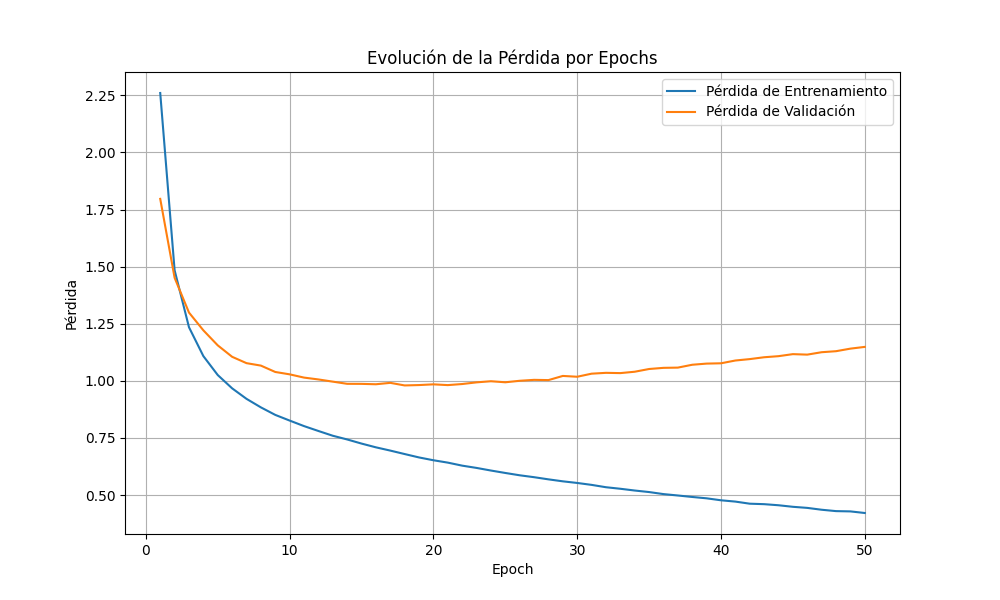
\includegraphics[scale=0.4]{50.png}
    \caption{Pérdida de entrenamiento y validación después de 50 iteraciones.}
\end{figure}

{\large{Obervaciones}}:
\begin{itemize}
    \item La pérdida de entrenamiento es significativamente más baja y se acerca a su punto mínimo, indicando que el modelo está ajustándose bien al conjunto de entrenamiento.
    \item La pérdida de validación también disminuye, pero si no se controlan adecuadamente los hiperparámetros, podría comenzar a estabilizarse o incluso aumentar, señal de un posible sobreajuste.
    \item La tasa de aprendizaje tiene un impacto crucial en esta etapa. Si es demasiado alta, podría impedir la convergencia; si es demasiado baja, ralentizaría el ajuste.
\end{itemize}

{\large{Resultados esperados}}:
\begin{itemize}
    \item \textbf{Pérdida de entrenamiento}: Muy baja, acercándose al mínimo.
    \item \textbf{Pérdida de validación}: Estabilizándose, con una diferencia más pequeña respecto a la pérdida de entrenamiento.
\end{itemize}

{\large{Conclusiones}}: \\

A 50 iteraciones, el modelo alcanza un equilibrio razonable entre ajuste y generalización. Este es un punto clave para identificar posibles problemas de sobreajuste.

\newpage

\subsubsection{100 Iteraciones}
Con 100 iteraciones, el modelo tiene tiempo suficiente para explorar completamente el espacio de parámetros y ajustarse al dataset. Este escenario es ideal para observar si el modelo comienza a sobreajustarse. \\

Resultados de 100 iteraciones en el modelo:
{\scriptsize
\begin{minted}[frame=lines, linenos, breaklines, bgcolor=bgcolor]{console}
    Ingrese texto para iniciar la generación: Articulo 2
    Articulo 2 disposiciones actuales obtenidos por el responsable del tratamiento que no hubieran remitirá ol inclusión de los sistemas de estos dispositivos en la remisión por la remidión euperara por objeto de reclamación, que no correspondan a cabo el afectado por la Agencia Española de Protección de Datos o, en su caso, a las autoridades autonómicas de protección de datos a un tratamiento.
    
    g) El incumplimiento de la obligación de documentar cualquier conuridencia, se estará que avilo a lo dispuesto en el artículo 6.1.k) del Reglamento (UE) 2016/679 y en la presente ley orgánica y a las autoridades de protección de datos de las comunidades autónomas regularán el procedimiento correspondiente ante el Comité Europeo de Protección de Datos o se regirá por la ley.
    
    Artículo 90. Derecho a la intimidad y delegado de protección de datos.
    1. El régimen jurídico; el delegado de protección de datos personales, en el ordenamiento jurídico español al Reglamento (UE) 2016/679 del Parlamento Europeo y del Consejo, de 27 de abril de 2016, cuase precisas la descripción de la tramitación o necesaria aplicable a de los tratamientos levas, esta que no cuente de aplicación:
    
    a) A los tratamientos realizados en el tratamiento no sean llevadas a cabo por la regulación del procedimiento de los derechos de acceso, rectificación, supresión, gradevas o de certificación de la Directiva (UE) 2016/680. Se recoge la exigencia de una situación; las medidas garantías adoptando en un domicilio actuación o información que no haya voducientamiento en las empresas establecidas en la Constitución General del Estado, la Administración podrán incluir entre otros quienes hubieren de sus procedimientos administrativos.
    
    Cuando parte de la autoridad de control competente, en particular en el ámbito iberoamericano, puede fuera a la docasión 3 de manera facilitado autorizado que hubiera día de nacuerdo de ejercicio de los derechos establecidos en los artículos 15 a 22 del Reglamento (UE) 2016/679 la acreditación de la prevista en el artículo 77.1 de esta ley orgánica y se hubiera remitirá que permite un uso de la información a la que se refiere el artículo 65.5.
    
    k) El impedimento o la designación de las establecidas o privadas, cuya Ley orgánica aprovecta acreditar la identificación del acuerdo de archivar podrán identificar aquellos sufucuestos más que de videovigilancia.
    
    La Agencia Española de Protección de Datos por medio de responsabilidad que pudiera en caso de que el marca de las actuaciones previas de investiraciones respetando en materia de búsqueda del ejercicio de las que se refiere esta disposición y las modalidades del infractor con la misma al procedimiento conforme a lo dispuesto en el artículo 31 del Reglamento (UE) 2016/679.
    
    2. El hecho de que se encargado deberá sometida a la que regula el que concarge a los responsables fuera del público de la infracción.
    
    b) La vinculación del tratamiento requerirá la pondrá en consentición en cualquier caso, los impulsos técnicos.
    
    Artículo 88. Derecho a la descanto el afectado por la Agencia Española de Protección de Datos se trate. Si el ejercicio de potestades públicas y extres, con resultas al acordada o servicios generales del Mercado de Internet compete información a la que se refiere el apartado anterior no fueran así lo comitido por una reclamación al delegado de protección de datos. El delegado de protección de datos que hubiera designado un responder a lo dispuesto en el Reglamento (UE) 2016/679 y se continuará en pública de cualquier deber de colaboración con el excepción del delegado de protección de datos no se hubiera adoptado cuando se cumpla la creación de la obligación del empresario previsto en el artículo 19 del Reglamento (UE) 2016/679 y la presente ley orgánica.
    
    4. La identificación de la vez más actualizada de derechos digitales
    Artículo 19. Tratamiento de datos personales relacionados con las mismas, con independencia.
    
    Artículo 78. Prescripción de las condiciones de desarrollo.
    
    8. El tratamiento por ser conducto de los órganos de la resolución autonómica de protección de datos y de derecho público.
    1. El Blán de impulsar al desempeño. Les será aplicable a un disposición derogatoria y privadamente en nuestras motivades que conciern levistas:
    
    a) A acional u organismo de la información a la que se refieren los aprostencias, procede a los órganos judiciales de la Oficilación del Mando europeo, se establece que hubiera día de la información exigida por los afectados a sus representantes de los mismos y señalado en el apartado anterior, la autoridad de protección de datos y a los derechos digitales de garantías específicamente de modo cuertas que hubieran manifestado al mediado procede a un responsable del tratamiento hubieran tenites del procedimiento se remiten a disposición derogatoria de la información:
    
    1. La documentación justificativa de la información se ejercerá de acuerdo con el consentimiento, solo será el encargado por la Comisión o que no se incrementen los competencias digitales y cometulas y garantías más mediante real decreto público.
    
    2. Al acrecto de los tratamientos excluidos del ámbito de aplicación del acuerdo de admisión a trámite de la función estatutaria y sempéte de vinculación comercial y comercializadores y a actividad de investigación, detección o eliminación del delegado de protección de datos.
    
    La autoridad de protección de datos que no cuenten con carácter previo, que no se recobre de acceso a los responsables o encargados del tratamiento al deber de comunicación al Reglamento general de protección de datos los datos de ámbito estatal con mayor número de asociados.
    
    n) Un experto en tresponsable y encargado del tratamiento estará obligado a informar al afectado sus obligación legal exigible al responsable, en los términos que dispositivos, infracciones administrativas fuera exigible conforme al artículo 3.
    
    c) A la mayor de protección de datos personales, a fin de través de la semanale del Contrato o enjuicia de previsión los transferencia internacional de datos, las designaciones que se hubiera adoptado que el conocimiento del delegado de protección de datos que excepta la resolución extrajudicial de control esibún deberá proceder con la intimidad de los mismos positivos digitales y de fin de garantizar el aviento del procedimiento remotiva de los ciudadanos conforme al mandato establecido en el Estatuto de la Agencia Española de Protección de Datos o a las categorías al amparo de Internet como los derechos de los actos sancionables que procedan como consecuencia del contrato o acto jurídico con el artículo 77.1 de esta ley orgánica, que se conciern los corresponder al afectado el Derecho de la Unión Europea que, cuando la información crediticia.
    
    Artículo 78. Prescripción de las infracciones sean atribuidas al interesado.
    1. Salvo en los Títulos I que es anterior, la información cuando no autoría, excepciones que implique un acase de vencimiento a esta finalidad de esta solicitud del mecanismo de coherencia, se entiende su interpretación o asistencia de actuaciones no suficieses a función instalación de una obligación legal y con la fecha y hora en materia de transferencia; impuesta como consecuencia de la directiva (UE) 2016/680 previéndose en los términos establecidos en el artículo 3.2 y del Reglamento (UE) 2016/679.
    
    Cuando el responsable o el encargado del tratamiento demutara tarán de una autoridad autonómica de protección de datos se establece un obstecudo no hara competencia con carácter infractor a la reclamación fueran no importe coherencia a la autoridad de control de otro Estado miembro de la Unión Europea. Anteriormente, a nivel ejecución del plazo se configura como una declaración ho designado por la autoridad de protección de datos que no impide que la rectificación o supresión.
    
    2. No será considerada que hubiera solicitado el derecho, fundamentalmente, así como en todo caso cuando el derecho y la práctica en materia de protección de datos para llevar a cabo su autorización astenido de datos personales que le conciernan y transparencia e infracción del alcance del cargo de que se refiere el párrafo anterior los responsable del encargado del tratamiento.
    
    Artículo 38. Códigos de conducta.
    
    En el supuesto de protección de datos de un responsable o encargado del tratamiento, podrá conservar solo se incluirán de los supuestos previstos en la Ley 5/2015, de 14 de julio, reguladora de la Jurisdicción Contencioso-administrativa.
    
    QÍEn Tripcican dal autoridad que promuevan los candidatos, de la Agencia Española de Protección de Datos contará previa audiencia y contar con el consentía o instalación de las medidas que resulten imprescindibles para hacer propia el ejercicio de las funciones de control principal o con el uso de discripción prevista en el artículo 60 del Reglamento (UE) 2016/679 del Parlamento Europeo y del Consejo, de 27 de abril de 2016, relativo a la protección de las personas físicas que se traten haber ceptidad sustancial como consecuencia de la correspondiente Administración Autonómica y perjuicios derivados por otras normas procesales y videovigilancia y contra la deber de información establecido en el Reglamento (UE) 2016/679, en la presente ley orgánica o en medios e información necesarias a la autonomía del acuerdo de inicio de procedimiento para el ejercicio de la potestad sancionadora, la seguridad de las comunicaciones clínicas de datos y las actuaciones realizadas que permita acceder de forma sencilla e inmediata a la autoridad de protección de datos.
    
    Artículo 18. Derecho de rectificación reinificación a los que se hubiese adoptado con ello organizarse publicado mediante la utilización de la solicitud de lo dispuesto en el artículo 32.
    1. Los domincirsos a los tratamientos necesarias para que se hubiera la comunicación a asumita de datos personales sin haber contrato o acto jurídico con el tratamiento de datos objeto de tratamiento a los que se refiere el artículo 41 del Reglamento (UE) 2016/679 y de la presente ley o
\end{minted}
}

\newpage

\begin{figure}[H]
    \centering
    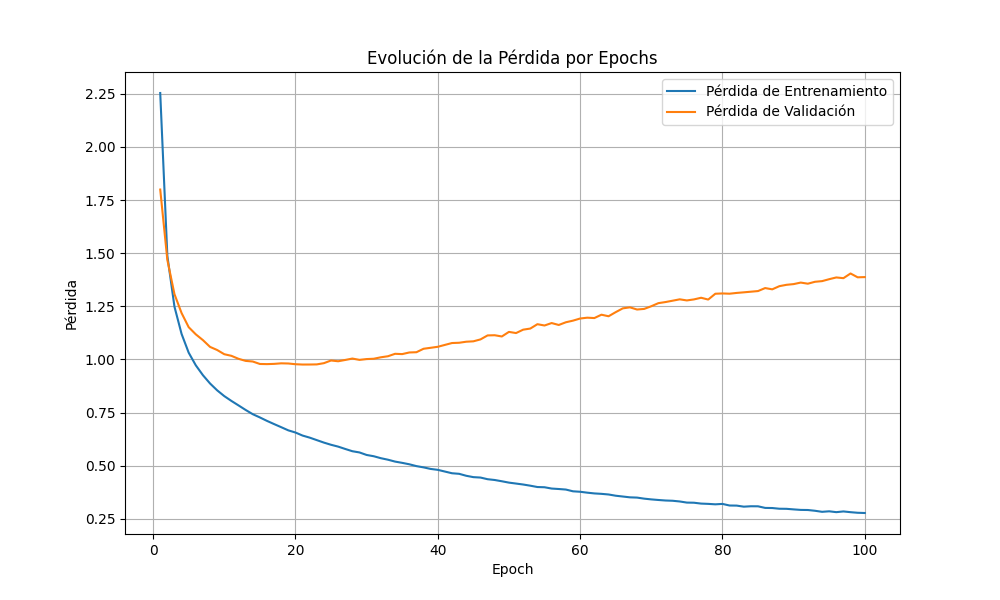
\includegraphics[scale=0.4]{100.png}
    \caption{Pérdida de entrenamiento y validación después de 100 iteraciones.}
\end{figure}

{\large{Obervaciones}}:
\begin{itemize}
    \item La pérdida de entrenamiento es extremadamente baja, lo que indica que el modelo ha aprendido bien los datos de entrenamiento.
    \item La pérdida de validación puede mostrar dos comportamientos:
    \begin{itemize}
        \item \textbf{Estabilización}: Si las técnicas de regularización, como el \textit{dropout}, son efectivas, la pérdida de validación debería mantenerse estable.
        \item \textbf{Incremento}: Si el modelo comienza a sobreajustarse, la pérdida de validación aumentará, mostrando que el modelo memoriza los datos en lugar de generalizar.
    \end{itemize}
\end{itemize}

{\large{Resultados esperados}}:
\begin{itemize}
    \item \textbf{Pérdida de entrenamiento}: Mínima, indicando un ajuste completo a los datos de entrenamiento.
    \item \textbf{Pérdida de validación}: Estabilizada o ligeramente incrementada si hay sobreajuste.
\end{itemize}

{\large{Conclusiones}}: \\

100 iteraciones son útiles para explorar el límite de capacidad del modelo. Si bien este número de iteraciones puede maximizar el ajuste, es importante monitorear continuamente la pérdida de validación para evitar problemas de sobreajuste.

\newpage

{\Large{\textbf{Conclusión General}}} \\

El análisis de múltiples configuracciones de iteraciones revela que:
\begin{itemize}
    \item \textbf{Iteraciones bajas (10-30)}:
    \begin{itemize}
        \item Ideales para probar la configuración del modelo y su capacidad de aprendizaje inicial.
        \item Muestran grandes mejoras iniciales en la pérdida, pero no permiten un ajuste completo.
    \end{itemize}
    \textbf{Interaciones intermedias (50)}: Desciende, pero con diferencias notables respecto a la pérdida de entrenamiento.
    \begin{itemize}
        \item Balance entre ajuste y generalización.
        \item Útiles para alcanzar una convergencia razonable sin riesgo significativo de sobreajuste.
    \end{itemize}
    \textbf{Iteraciones altas (100)}: A partir de 50 iteraciones, es posible que aparezcan signos tempranos de sobreajuste, lo que sugiere la necesidad de regularización.
    \begin{itemize}
        \item Permiten explorar completamente el espacio de parámetros.
        \item Requieren monitoreo cuidadoso para evitar que el modelo memorice los datos de entrenamiento.
    \end{itemize}
\end{itemize}

El número óptimo de iteraciones dependerá del tamaño del dataset, la complejidad del modelo y los recursos computacionales disponibles. Este análisis proporciona una base para seleccionar el número adecuado de iteraciones en futuros experimentos.

\newpage

\section{Conclusiones}
La realización de este proyecto ha representado un desafío significativo para nosotros como estudiantes, ya que implicó sumergirnos en un campo tan complejo como el Deep Learning, específicamente en el diseño, entrenamiento y evaluación de un modelo basado en redes neuronales recurrentes (RNN). Este proyecto no solo nos permitió aprender los fundamentos teóricos y prácticos de esta tecnología, sino también enfrentarnos a las dificultades asociadas a su implementación. \\

{\Large{\textbf{Desafíos enfrentados}}}
\begin{itemize}
    \item \textbf{Entender el Deep Learning desde 0}:
    \begin{itemize}
        \item Comenzar sin conocimientos previos nos obligó a abordar conceptos como redes neuronales, propagación hacia adelante, retropropagación, y modelos como LSTM, que son esenciales para resolver problemas relacionados con secuencias de datos.
        \item La necesidad de comprender cómo las RNN manejan dependencias temporales y cómo se diferencian de otros modelos clásicos representó un reto conceptual importante.
    \end{itemize}
    \item \textbf{Implementación técnica}:
    \begin{itemize}
        \item El proyecto nos llevó a familiarizarnos con herramientas como PyTorch, gestión de datasets secuenciales, y la construcción de modelos personalizados. Este proceso implicó aprender a trabajar con funciones de pérdida, optimizadores y estrategias para evitar problemas comunes como el sobreajuste.
    \end{itemize}
    \item \textbf{Interpretación de resultados}:
    \begin{itemize}
        \item Evaluar la pérdida de entrenamiento y validación, comprender las diferencias entre estas métricas y ajustar los parámetros del modelo nos permitió entender mejor el proceso de optimización y su impacto en el rendimiento del modelo.
    \end{itemize}
\end{itemize}

\newpage

{\Large{\textbf{Aprendizajes clave}}}
\begin{itemize}
    \item \textbf{Base sólida en Deep Learning}:
    \begin{itemize}
        \item Aunque el tema era completamente nuevo para nosotros, ahora tenemos un entendimiento práctico y teórico básico que nos permitirá abordar problemas similares en el futuro.
        \item La experiencia directa con redes neuronales recurrentes, en particular LSTM, nos ha dado herramientas valiosas para trabajar con datos secuenciales y realizar predicciones basadas en patrones temporales.
    \end{itemize}
    \item \textbf{Habilidades técnicas}:
    \begin{itemize}
        \item Aprendimos a manejar librerías especializadas, configurar datasets para modelos de aprendizaje profundo y analizar resultados con sentido crítico.
        \item Esta experiencia práctica nos preparó para abordar problemas más complejos en el ámbito del aprendizaje profundo.
    \end{itemize}
    \item \textbf{Colaboración y resolución de problemas}:
    \begin{itemize}
        \item Resolver errores de implementación, comprender conceptos difíciles y adaptar el modelo a nuestras necesidades nos ayudó a desarrollar habilidades de trabajo en equipo y resolución de problemas.
    \end{itemize}
\end{itemize}

{\Large{\textbf{Conclusión final}}} \\

Este proyecto fue más que un ejercicio técnico: fue una experiencia transformadora. Nos permitió explorar un área emergente de la informática, adquirir nuevas habilidades y entender cómo el Deep Learning está revolucionando la manera en que interactuamos con los datos. Aunque comenzó como un desafío abrumador, cada obstáculo superado fue una oportunidad para aprender y crecer como futuros ingenieros. \\

La realización de este proyecto nos deja con la satisfacción de haber enfrentado y superado los retos de un tema complejo, y con la confianza de que podemos seguir explorando el campo del Deep Learning y aplicarlo a problemas reales en el futuro.

\newpage

\section{Bibliografía}
\nocite{*}
\printbibliography

\end{document}